% Note that the a4paper option is mainly intended so that authors in
% countries using A4 can easily print to A4 and see how their papers will
% look in print - the typesetting of the document will not typically be
% affected with changes in paper size (but the bottom and side margins will).
% Use the testflow package mentioned above to verify correct handling of
% both paper sizes by the user's LaTeX system.
%
% Also note that the "draftcls" or "draftclsnofoot", not "draft", option
% should be used if it is desired that the figures are to be displayed in
% draft mode.
%
\documentclass[conference, compsoc]{IEEEtran}

% Add the compsoc option for Computer Society conferences.


\usepackage{url} 
\usepackage{times}
%For math symbols like number classes
\usepackage{amsfonts}
\usepackage{amssymb}
%\usepackage{amsthm}
\usepackage{floatflt}
\usepackage{wrapfig}
\usepackage{multirow}

\usepackage[T1]{fontenc}
\usepackage{hyperref}
\usepackage[cmex10]{amsmath}
\usepackage{acronym}
\interdisplaylinepenalty=2500
\usepackage{xspace} % noget med mellemrum efter forkortelser
\usepackage{longtable}
\usepackage[pdftex]{graphicx}
\usepackage[pdftex]{graphics}

\usepackage[boxed,linesnumbered,vlined,slide]{algorithm2eCustom}

%\usepackage{epstopdf}
%\DeclareGraphicsExtensions{.pdf,.eps,.png,.jpg,.mps}

%\ $[\today]$
% *** CITATION PACKAGES ***
%
\usepackage{cite}


% correct bad hyphenation here
\hyphenation{op-tical net-works semi-conduc-tor}


\begin{document}
\newcommand{\ffh}[1]{\textbf{TODO: \textit{#1}}} 
\newcommand{\baseline}{Baseline \xspace} 
\newcommand{\dynamgrid}{Dynamic Grid \xspace}
\newcommand{\md}{\mdns \xspace}
\newcommand{\mdns}{MD}
\newcommand{\mds}{\mdsns \xspace}
\newcommand{\mdsns}{MDs}
\newcommand{\ls}{\lsns \xspace}
\newcommand{\lsns}{LS}
\newcommand{\lss}{\lssns \xspace}
\newcommand{\lssns}{LSs}
\newcommand{\ff}{\ffns \xspace}
\newcommand{\ffns}{\textsc{FriendLocator}}
\newcommand{\ffs}{\ffsns \xspace}
\newcommand{\ffsns}{\textsc{FriendLocators}}
\newcommand{\hc}{\hcns \xspace}
\newcommand{\hcns}{\texttt{Hide\&Crypt}}
\newcommand{\vl}{\vlns \xspace}
\newcommand{\vlns}{\textsc{VicinityLocator}}
\newcommand{\vls}{\vlsns \xspace}
\newcommand{\vlsns}{\textsc{VicinityLocators}}
\newcommand{\lmg}{\lmgns \xspace}
\newcommand{\lmgns}{LMG}
\newcommand{\lmgs}{\lmgsns \xspace}
\newcommand{\lmgsns}{LMGs}
\newcommand{\ttslong}{\ttslongns \xspace}
\newcommand{\ttslongns}{Trusted Third-party Server}
\newcommand{\tts}{\ttsns \xspace}
\newcommand{\ttsns}{TTS}
\newcommand{\iuns}{IU}
\newcommand{\rfns}{RF}
\newcommand{\iu}{\iuns \xspace}
\newcommand{\rf}{\rfns \xspace}
\newcommand{\iusns}{IUs}
\newcommand{\rfsns}{RFs}
\newcommand{\ius}{\iusns \xspace}
\newcommand{\rfs}{\rfsns \xspace}


\newcommand{\lpar}{(}
\newcommand{\rpar}{)}

\SetKwBlockLRS{LRSBegin}
\newcommand{\funcc}[3]{\emph{\textbf{#1}}\ensuremath{\lpar #2 \rpar} \LRSBegin{#3}}
%\newcommand{\func}[2]{\emph{\textbf{#1}}\ensuremath{\lpar #2 \rpar} \\}


%To change extension of algorithm2e use \algoext{A}, \algoext{B}, \Algoext{}
\newcommand{\algoext}[1]{\renewcommand{\thealgoext}{#1}}
 
 

 
 
%25000	2685185
%50000	4925925
%75000	7129629
%100000	9574074
\newtheorem{thm}{Theorem}[section]
\newtheorem{cor}[thm]{Corollary}
\newtheorem{lemma}[thm]{Lemma}
\newtheorem{deff}[thm]{Definition}
% \newenvironment{definition}[1][Definition]{\begin{trivlist}
% \item[\hskip \labelsep {\bfseries #1}]}{\end{trivlist}}

\SetKwBlockLRS{JRBegin}
\pagestyle{plain}

% paper title
% can use linebreaks \\ within to get better formatting as desired
\title{Fall 2010 \\ {\textit{\small \today}}}


\author{\IEEEauthorblockN{Jeppe Rishede Thomsen%\IEEEauthorrefmark{1},
\IEEEauthorblockA{%\IEEEauthorrefmark{1}
Department of Computing\\ Hong Kong Polytechnic University
}}}


\maketitle

%\acrodef{acronym}{definition}
\acrodef{MD}{Mobile Device}

\acrodef{CFG}{Context-Free Grammar}

\acrodef{CNF}{Chomsky Normal Form}

\acrodef{BNF}{Backus-Naur Form}

\acrodef{EBNF}{Extended Backus-Naur Form}

\acrodef{AST}{Abstract Syntax Tree}

\acrodef{LALR}{Look-Ahead Left-to-Right}

\acrodef{CLR}{Common Language Runtime}

\acrodef{CTS}{Common Type System}

\acrodef{IDE}{Integrated Development Enviroment}

\acrodef{LoC}{Lines of Code}

\acrodef{GUI}{Graphical User Interface}

\acrodef{UI}{User Interface}

\acrodef{AS} {Always Sensitive} 

\acrodef{ASTI} {Always Sensitive with time interval} 

\acrodef{ASST} {Often Sensitive at specific time}
	
\acrodef{RS} {Rarely sensitive}

\acrodef{PSR} {Potential Sensitive Region}

\acrodef{RT} {Road Type}

\acrodef{SSSP} {Single Source Shortest Path}

\acrodef{SP} {Shortest Path}

\acrodef{OSC} {Optimal Substructure Cache}

\acrodef{SPS} {\spath subpath Sharing}
\begin{abstract}
% All the papers either solve the problem of a more efficient cache in a specific domain, or use the network domain,  which are both relevant, but not really useful when looking at shortest path caching.
% 
% The papers show some interesting ways to use cache, but ultimately their approaches are very domain or query specific so their approaches to caching and cache replacement/invalidation can not be applied directly.


short description of what we do, why this is an interesting/challenging problem, and how well we solve the problem (key results, mention theoretical guaranties.)
\end{abstract}


% For peerreview papers, this IEEEtran command inserts a page break and
% creates the second title. It will be ignored for other modes.
\IEEEpeerreviewmaketitle



\section{Introduction} \label{sec:intro}

\subsection{idea for running example}
A user issues two queries as seen in fig. \ref{fig:advancedroutequery}. We can then argue, using this figures and the map in fig. \ref{fig:map10} about all the optimizations we plan to use. (same queries in all figures, and they correspond to map)




\section{Motivation}
Previous work on caching focus on domains which usually has two key characteristics: data locality and limited set of possible items which can be cached (\cite{ref.}). 
There has not been any previous work done developing a caching scheme usable in domains with large set of possible cacheable items and little or no locality in new items added to system, or suggested added to cache. \spath caching is one such domain.. 

\spath calculation is much slower than retrieval from cache, as a cache can supply a \spath directly. 
%where a \spath algorithm will on at most have to visit $AF^{AVN}$ nodes (see table of notation). 
\spath service providers want to spend less money on hardware (\cite{ref.}) and users want fast response time which (\cite{ref.}), when compared to investing in more hardware and bandwith, can be archived in a much cheaper and scalable way by implementing a \spath cache.

Returning a precomputed \spath result is faster, however, it is not feasible to store all possible \spaths. The cache replacement policy of a \spath cache ensures that most queries can be answered by the cache, ensuring as many queries as possible is answered with the space available to the \spath cache.

More users now have a GPS and Web enabled mobile devices which makes \spath services more popular, but also require them to serve much larger set of users.








% 
% \subsubsection{OSC - Optimal Substructure Cache}
% OSC is more advanced than the two previous proposed solutions and therefor the scenario has been updated in figure . 
% To further improve upon Improved Baseline we will again utilize the optimal substructure, making it possible to have much fewer items in cache and still retain a high cache hit percentage \cite{ref}. %(assumption, need test result or proof), 
% Results with sub-paths shared by many users and longer, rather than short, paths are preferred to increase the utility of the cached shortest-path results.
% 
% By adding a more intuitive cache replacement policy which takes in to consideration both the usage of each cache item, as well as the coverage of previously often seen queries it is likely that the utility of the cache would be much higher. This addition is shown with the addition of the "`add to cache"' box in figure \ref{fig:advancedroutequery}B, added to show a heuristic\footnote{the actual heuristic will of cause only be defined later} will be used instead of a very simple method like LRU.


%\paragraph{\textbf{Number 3, ideas}}
%use optimal substructure\\
%prefer having longer paths in cache\\
%prefer having paths with subpaths shared by many users\\
%look at utility of cache items, not just usage when designing cache replacement policy.\\
%\begin{itemize}
%\item	prefer often used cache items
%\item	prefer items which cover routes/areas often used in previous queries
%\end{itemize}





%\paragraph{crap}
%We assume a setting where all users are equipped
%with a Mobile Device (MD) able to communicate and
%report the users position. All MDs are online and are
%continuesly reporting the users location at predetermined
%intervals. We use the terms user, mobile device, and
%client interchangeable and denote the set of MDs by
%UN. We expect a MD to be cabable of visualizing
%its current location.
%We assume a 2D scenario, where the movements of
%users uU are restricted to a road network G(V, E).
%V is the set of vertices, where each vertice v ∈ V
%represents either a street intersection or an important
%landmark. E is the set of directed edges augmented
%by edge length and type. Edges are represented by
%a begin/end vertice pair and each edge represents the
%smallest unit of a road segment. e ∈ E, each e being
%a tuple specifying id, start-/end-vertices, length, and
%Road Type (RT) (eid , vs , ve , elength , eRT ). RT is a
%hierarchy of the size/type of road i.e. highway, paved,
%or dirt road (Sec. 5.2).
%The simplest form of trajectory is a collection of tu-
%ples (time, longitude, latitude), ordered by the time
%attribute, but as we will work on a road network and
%in the spatio-temporal domain, such a basic notion of
%trajectories is not appropriate. We define T as the set
%of trajectories, where each trajectory consist of an id
%(tid ), and a sequence of tuples containing an edge and




% \section{Related Work} \label{sec:rel_work}
%
In this section we review general location privacy preserving techniques 
followed by the relevant work on location privacy in proximity detection
services.

\subsection{General Location Privacy Techniques}

In the most common setting assumed in location-privacy research,
an LBS server maintains a public set of points-of-interest (POI), e.g. gas
stations. The goal is then to retrieve from the server the nearest POIs to the
user, without revealing the user's location $q$ to the server. Many
location privacy solutions exist for this setting and they can be broadly
classified into two categories: spatial cloaking and transformation. 

Spatial cloaking \cite{gruteser03,mca06,duckham05a,acdvs07} techniques
generalize the user's exact location $q$ into a region $Q'$, which is then used
for querying the server. The region $Q'$ is then sent to the LBS server, which
returns all the results that are relevant to any point in $Q'$. Such technique
ensures that even if the attacker knows locations of all users, the identity of
the querying user can be inferred only with some probability. 

The transformation approaches \cite{ks07,ghinita08} map the user's location $q$
and all POIs to a transformed space, in which the LBS server evaluates queries
blindly without knowing how to decode the corresponding real locations of the
users.

In contrast, in the proximity detection problem, the users' locations are both
query locations and points-of-interest that must be kept secret. Thus the
existing spatial cloaking and transformation techniques, that assume public
datasets, cannot be directly applied for proximity detection. However the
concepts of spatial cloaking and transformation can be, and are used in the
existing privacy-aware proximity detection approaches.

\subsection{Privacy-aware proximity detection methods}

Ruppel et al. \cite{proxDetTrans} develop a centralized solution that supports
proximity detection with a certain level of privacy. It applies a distance-preserving 
mapping (a rotation followed by a translation) to convert the user's location $q$ into 
a transformed location $q'$. Then, a centralized proximity detection method is 
applied to detect the proximity among those transformed locations. However, Liu 
et al. \cite{lgk06} points out that such distance-preserving mapping is not safe 
and a attacker can easily derive the mapping function and compute the users' original 
locations. 

% maybe remove???
Mascetti et al. present a centralized solution
\texttt{Longitude} \cite{longitudePaper}.
Here users apply spatial cloaking followed by modular transformation prior
sending their 
locations the server. The applied transformation prevents the disclosure of 
location information, but introduces false proximity detections that do not occur in our 
proposed approach.


\hc, presented in \cite{pbsPaper}, is a privacy preserving solution which employ
the filter-and-refine paradigm. First, users spatially cloak their locations and sent them the
server. Then, the server computes a minimum and maximum distances (Fig. \ref{fig:relworkDemos}a)
between these cloaking regions. Depending on the specified thresholds and computed distances, 
the server classifies friends being in, not-in, or possibly-in proximity. The classification 
result is immediately reported to users, and in case of uncertainty, two users have to perform 
direct communication in order to refine their proximity status. 
In the refinement step first two users map their locations 
and vicinity regions into the some spatial subdivision, e.g. grid, and then they use secure 
two-party computation protocol to check if the mapped location of one user lays inside the 
mapped vicinity of other user. This can be performed with no need for the users 
to expose their mapped locations and vicinities. Depending on the result of the 
set-inclusion checking, either proximity or separation is detected. Figure
\ref{fig:relworkDemos}b visualizes a scenario, where user $u_2$'s grid-mapped location
(dark rectangle) intersect with $u_1$'s grid-mapped vicinity region. In this case, 
the proximity between $u_1$ and $u_2$ is detected.

Unlike in our approach, their proposal does not completely hide user locations
from the central server as it always knows their cloaked regions. If strong
privacy is required users are forced to perform user-to-user communication more
frequently thus significantly increasing the amount of client communication due to
an expensive secure two-party computation protocol. 



\begin{figure}
       \center
       \begin{tabular}{cc}
			   
\includegraphics[width=0.25\textwidth]{vl/images/pbsDemo.pdf} &
			   
\includegraphics[width=0.18\textwidth]{vl/images/pbsDemo2.pdf} \\
%	Filtering step & Refinement step \\
          (a) & (b) \\
\includegraphics[width=0.15\textwidth]{vl/images/proxDetDemo.pdf} &
{\scriptsize %\footnotesize
     \begin{tabular}[b]{| c | c |}\hline
        \textbf{Col/ Row} & \textbf{$\mathbf{\Psi}$} \\  \hline
        0 & $c_0$ (5)\\ \hline
        1 & $c_1$ (9)\\ \hline
        2 & $c_2$ (1)\\ \hline
        3 & $c_3$ (7)\\ \hline	
     \end{tabular}
} \\
          (c) & (d)
       \end{tabular}
       \caption{Behavior of \hc and \ff}
            \label{fig:relworkDemos}
\end{figure}



\v{S}ik\v{s}nys et al. \cite{ffinder} have developed a centralized privacy-aware
proximity detection method, called \ff, which provides strong privacy guaranties
and employs a grid-based technique to optimize communication cost. 
Users map their locations into 4 cells of the grid from a \textit{list of grids},
and, prior sending to the server, encrypt them using shared, one-to-one mapping encryption function.
The \textit{list of grids} globally defines a collection of grids, where cell sizes of distinct grids 
monotonically decreases with respect to the \textit{level number}. The server is able to 
perform a matching between encrypted coordinates of different users, for a shared
level, and report the matching result. When matchings at all consecutive levels 1
to $L_{max}$ are detected then actual proximity between two users is detected.
Pairs of users individually choose $L_{max}$ value which yields a
specific mutual vicinity radius for two users. The proximity is detected
iteratively such that after each encrypted coordinate match, 
the server checks if required level $L_{max}$ is reached. If so, then users are
informed about their proximity, otherwise the server sends a message to one or
both of the users asking them to use a finer grid, i.e., increase their current
level, for the next matching iteration. 

E.g. if the encryption function $\Psi$ is as defined in
\ref{fig:relworkDemos}d, then encrypted coordinates of users $u_1$, $u_2$, and
$u_3$ respectively are $(x:[c1,c2],y:[c0,c1])$, $(x:[c2,c3],y:[c1,c2])$,
$(x:[c0,c1],y:[c2,c3])$. Assuming that level of grid in Fig.
\ref{fig:relworkDemos}c is $L_{max}$, the user $u_1$ is in proximity with $u_2$,
however $u_3$ is not in proximity with either.



The limitation of the \ff is low, and uncontrollable, precision of the
proximity detection. On the proximity notification the actual distance between
two users can be any in the range from $d$ to $d + \lambda$, 
where $d$ is width/height of grid cell at level $L_{max}$, 
$\lambda = d(2\sqrt(2) - 1)$ is a service precision parameter. Note, 
that in most other proximity detection approaches, unlike in \ff, the parameter 
$\lambda$ can be chosen freely by users. 

None of the existing privacy-aware approaches directly support the ``river'' 
and the ``bar'' proximity detection scenarios (see Fig. 
\ref{fig:suppVic}c/\ref{fig:suppVic}d) since they use static circular-shape vicinity. 
However some solutions, like \hc \cite{pbsPaper}, might be adapted to support dynamic 
vicinities, though current limitations will persist and introduce new problems 
like e.g. how to efficiently update user locations and vicinities.




\subsection{Our contribution}

In this work we combine best features of the previously presented proximity
detection approaches to build our solution, the \vl. The solution combines the
ideas of encrypted coordinates, their blind matching at the server-side, and
the vicinity mapping into multi-spatial subdivisions, e.g. list of grids.
Our solution, unlike Mascetti et al. \cite{pbsPaper} proposal, employs only
centralized architecture, where the server knows no users' spatial data. It
allows users individually select preferable proximity detection precision and 
supports irregular-shape, changing over time vicinities. Our proposal
is will be targeted for 2D environment.
It can however easily be generalized to n-dimension.

\section{Problem}\label{sec:problem}

In our setting we assume users own an Internet enabled mobile device with positioning capabilities. Users issue \spath queries to an online service provider. Users want the response time, on the return of their \spath result, to be comparable to that of an offline application. We use the terms user query, incoming query, and query interchangeably.

The \spath service provider needs to provide a fast service to its users. The service provider also want to save cost on hardware, such as CPU and HDD space. The \spath provider therefor wants to return as many \spath results as possible, using the least amount of computation and space.

Calculating a \spath will, regardless of the algorithm used, always be an expensive calculation\cite{CNeed}. Using a \spath cache at the \spath service provider can reduce the CPU cycles used in order to return a \spath result. Doing so would at the same time also increase the response time of the \spath service, as saving CPU cycles not only allows for more \spaths to be computed on the same hardware, but also allows for returning a cached result much faster than it would be possible if the \spath had to be calculated first.

A \spath has the property of \oss (see lemma \ref{lem:oss}) which means that any \spath in the cache can answer any \spath query where both origin and target node are on the \spathns. Calculating which \spathsns, and their sub-paths, provide the most benefit will obviously be necessary for optimal utilization of the cache. A static cache, which is populated in an offline phase (fig. \ref{fig:routequery}E), is used. A static cache will impose minimal overhead to query processing. Section \ref{sec:competitors} explains why we choose a static cache.

The properties of \ossns (Lemma \ref{lem:oss}) states that all sub-paths on a \spath are also \spathsns. Using \spath Q1 in table \ref{tab:queries} we would also be able to a query from $v_3$ to $v_5$, or $v_4$ to $v_6$ (See fig. \ref{fig:rxmap}), as these nodes are part of Q1. The same of cause also holds for any \spath Q1-Q6 from table \ref{tab:queries}.

\begin{figure}[hbt]
  \center
        \includegraphics[width=0.5\textwidth]{figures/rxmap}
        \caption{Simple graph representation of a map.}
  \label{fig:rxmap}
\end{figure}


\subsection{Architecture}
We propose a system with a static \spath cache implemented in front of an existing \spath service (See fig. \ref{fig:routequery}) such that if the cache can answer a query then the result can be returned immediately. 

When the system receives a \spath query from a user (fig. \ref{fig:routequery}A) the system first checks if the cache (fig. \ref{fig:routequery}B) is able to answer the query. If the cache contains the query answer it is immediately returned (fig. \ref{fig:routequery}D), else the \spath algorithm is called (fig. \ref{fig:routequery}C) and the \spath result returned (fig. \ref{fig:routequery}D).

\begin{figure}
  \center
        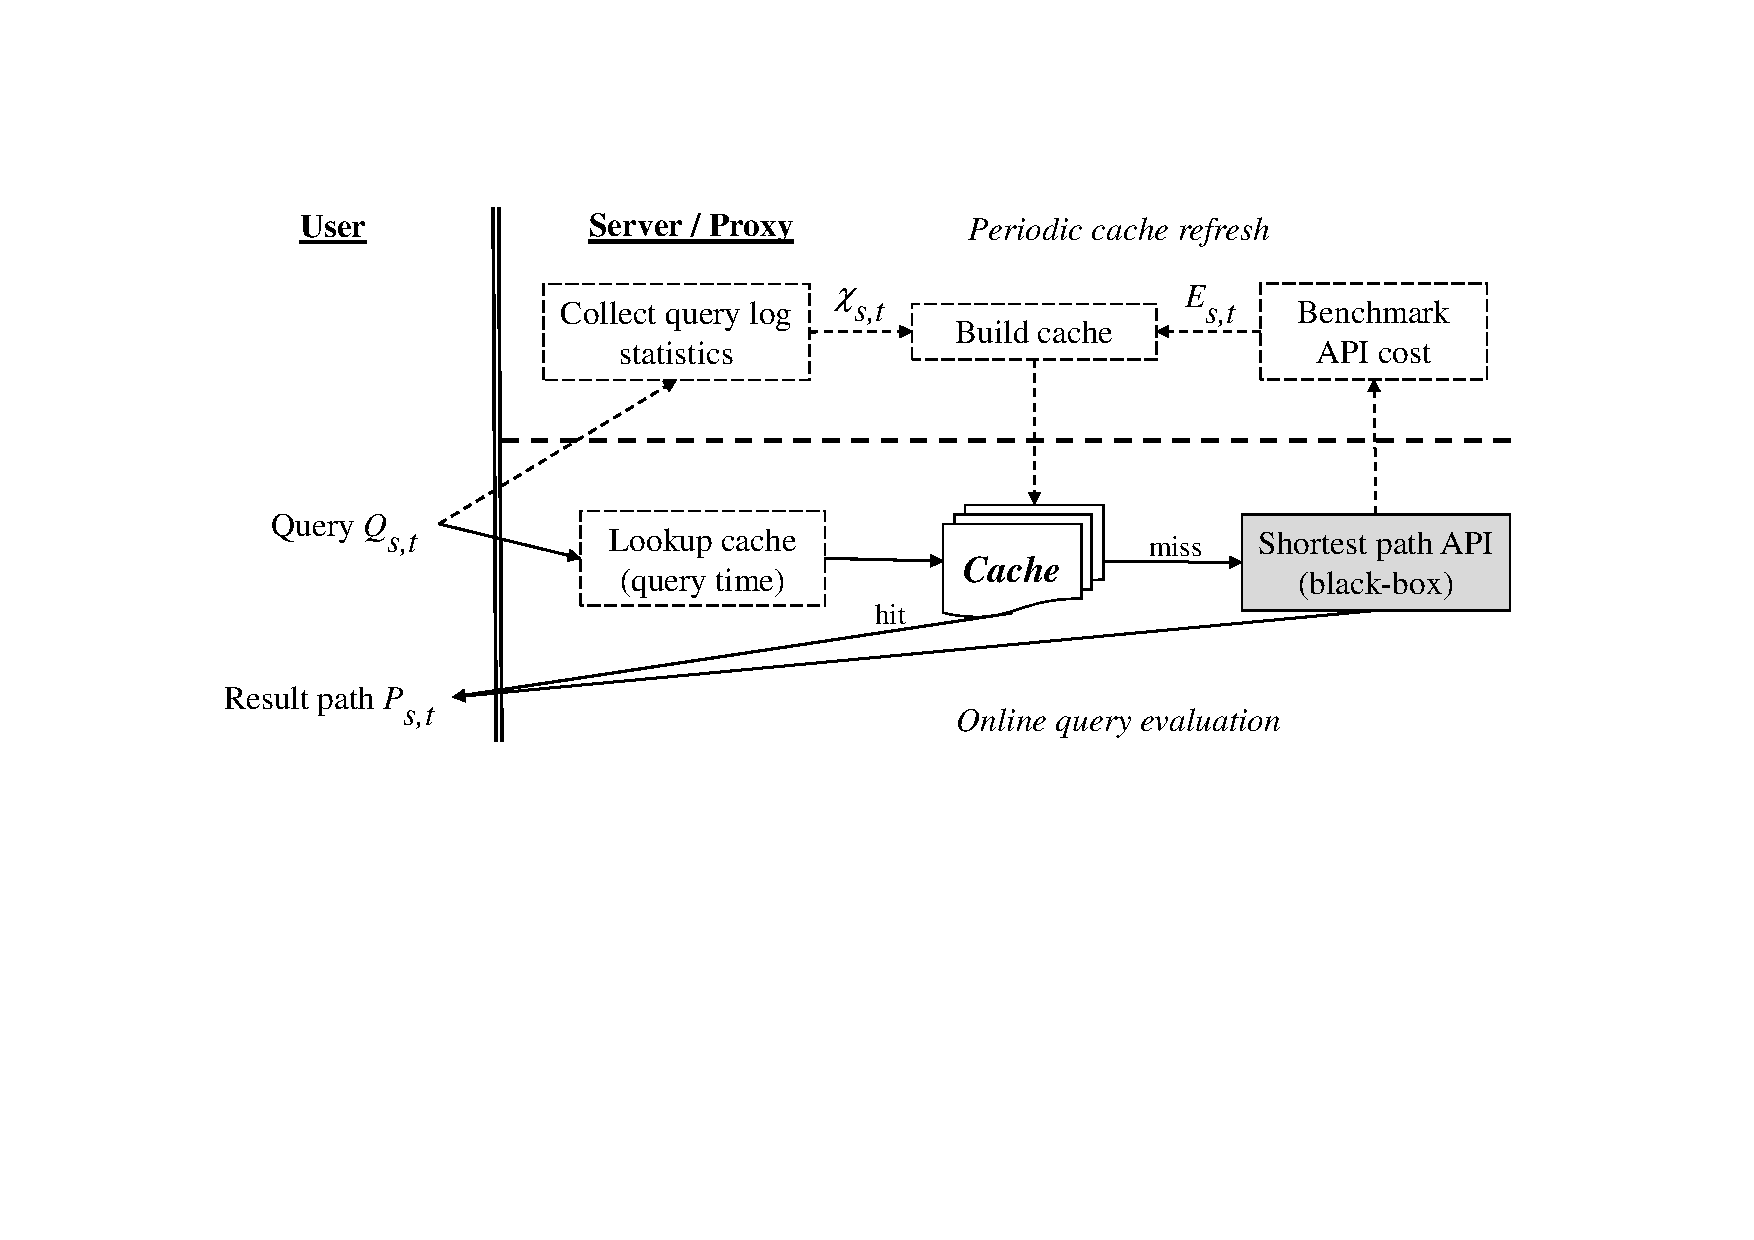
\includegraphics[width=0.5\textwidth]{figures/routequery}
        \caption{Buffer placement in \spath service providers system.}
  \label{fig:routequery}
\end{figure}


\subsection{Optimization Intend} \label{subsec:goals}

As the main problem with expensive \spath calculations is time needed, we use reduction in \textit{\cet} as the main optimization target and measurement to evaluate our success.
At a \spath service provider, the time spent to return a \spath result is essentially composed of two tasks: calculating the \spath and the overhead of query processing. 

We will address 3 subgoals:
\begin{enumerate}
\item \label{item:goal1}Reduce the gross \cet used to calculate \spathsns.
\item \label{item:goal2}Reduce the gross \cet spent on overhead in query processing.
\item \label{item:goal3}Determine the value of a sub-path in the cache.
\end{enumerate}

We want reduce the gross \cet of \spath calculations - goal 1 - as it is the most CPU intensive task at a \spath service, and therefor also the most time consuming. By using a cache we expect to see a negavite correlation between cache hit rate and \cet used on \spath calculation.

In a \spath service there will always be a some overhead associated with \spath query processing. Introducing a cache in front of the existing \spath service (fig. \ref{fig:routequery}B) will undeniably add more overhead as the cache needs to be queried for all queries submitted to the \spath service, regardless of whether it is able to answer the query or not. In order for the cache to be useful, the overhead introduced needs to be minimized (goal \ref{item:goal2}). We always have to make sure that the savings achieved by adding a cache to the system is greater than the overhead introduced.

The fact that the system will be using a static cache, and \spaths exhibit the \oss property, makes goal 3 - determining the value of a \spath subpath - very important. The ability to do goal \ref{item:goal3} well will have a direct influence on goal \ref{item:goal1} and  \ref{item:goal2}. If we fill the cache with useless \spaths we will end up calculating a \spath for all queries, as well as the overhead from checking the cache for each query. Solving goal 3 well is the most direct way to solve goal 1.

The \oss property states that every sub-path of a \spath is also a \spath. i.e \spath Q1 in table \ref{tab:queries} consists of: 
$\{Q_{1,3}, Q_{1,4}, Q_{1,5}, Q_{1,6}, Q_{3,4},$ $Q_{3,5}, Q_{3,6}, Q_{4,5}, Q_{4,6}, Q_{5,6}\}$, each one being a \spathns.

\begin{lemma}\label{lem:oss}
If a path $Q_{s,t}: v_s,v_{s+1},\ldots,v_t$ is a \spath, then $\forall$ $(v_k,v_l) | v_k \in Q_{s,t} \wedge v_l \in Q_{s,t}$ there is a  \spath $Q_{k,l}$ with start-/end-node in $v_k,v_l$, following a sub-path of $Q_{s,t}$ 
\end{lemma}

\begin{table}
\begin{tabular*}{\columnwidth}{|l||p{0.69\columnwidth}|}
\hline
\bf Abbreviation & \bf Meaning \\\hline
\spath          & Shortest Path \\\hline
$Q_{s,t}$	& \spathns: $\{v_s,v_{s+1},\ldots,v_t\}$ \\\hline
\acs{LRU}       & \acl{LRU} \\\hline
FIFO            & First In First Out \\\hline
\acs{SPS}       & \acl{SPS} \\\hline
\acs{CET}	& \acl{CET} \\\hline
\acs{OSS}	& \acl{OSS} \\\hline
\end{tabular*}
\caption{Table of Notation}
\label{tab:symbols}
\end{table}




% \subsection{helping text}
% \begin{enumerate}
% \item Introduce the problem setting in more detail than in the introduction and formally define the problem and what exactly we aim to solve in this paper.\\
% \item show where exactly the proposed cache is located in an online \spath service providers system.
% \item State goal 1(a) and 2(b)
% 	\begin{enumerate}
% 	\item Reduce the time spent executing the \spath algorithm. - The \spath algorithm is usually the single most CPU expensive task at a \spath service provider.
% 	\item Reduce the time spent on overhead. - Introducing a cache will also add some overhead, this overhead not desirable and should  be minimized.
% 	\end{enumerate}
% \item Introduce the overall setting which our solution work in and give a table of notation for reader reference.
% \end{enumerate}
%
\section{Contribution}

\subsection{Statistics Extraction}

\begin{frame}[shrink=10] %hmm.. thought i could change colour here :S
\frametitle{Statistics Extraction} 


    \begin{tabular}{ccc}
\begin{tabular}{@{}|c@{}|c@{}|@{}}
\hline
Timestamp & Query \\ \hline 
$T_1$ & $Q_{3,6}$ \\ \hline 
$T_2$ & $Q_{1,6}$ \\ \hline 
$T_3$ & $Q_{2,7}$ \\ \hline 
$T_4$ & $Q_{1,4}$ \\ \hline 
$T_5$ & $Q_{4,8}$ \\ \hline 
$T_6$ & $Q_{2,5}$ \\ \hline 
$T_7$ & $Q_{3,6}$ \\ \hline  
$T_8$ & $Q_{3,6}$ \\ \hline 
\end{tabular}
&
    \begin{tabular}{|@{ }c@{ }|@{ }c@{ }c@{ }c@{ }c@{ }c@{ }c@{ }c@{ }c@{ }|}
       \hline
       $\chi_{s,t}$	& $v_1$	& $v_2$	& $v_3$	& $v_4$	& $v_5$	& $v_6$	& $v_7$ & $v_8$ \\\hline
       $v_1$			& /	& 0	& 0	& 1	& 0	& 1	& 0	& 0	 \\
       $v_2$			& 0	& /	& 0	& 0	& 1	& 0	& 1	& 0	 \\
       $v_3$			& 0	& 0	& /	& 0	& 0	& 3	& 0	& 0	 \\
       $v_4$			& 1	& 0	& 0	& /	& 0	& 0	& 0	& 1	 \\
       $v_5$			& 0	& 1	& 0	& 0	& /	& 0	& 0	& 0	 \\
       $v_6$			& 1	& 0	& 3	& 0	& 0	& /	& 0	& 0	 \\
       $v_7$			& 0	& 1	& 0	& 0	& 0	& 0	& / & 0  \\
       $v_8$			& 0	& 0	& 0	& 1	& 0	& 0	& 0 & /  \\
       \hline
    \end{tabular}
	\\
    \end{tabular}\\

\hspace{10em}\includegraphics[width=0.55\columnwidth]{images/rxmap} 


\end{frame}

\begin{frame}[shrink=10] %hmm.. thought i could change colour here :S
\frametitle{Grouping} 

\begin{tabular}{lc}

    \begin{tabular}{|@{ }c@{ }|@{ }c@{ }c@{ }c@{ }c@{ }c@{ }c@{ }c@{ }c@{ }|}
       \hline
       $\chi_{s,t}$	& $v_1$	& $v_2$	& $v_3$	& $v_4$	& $v_5$	& $v_6$	& $v_7$ & $v_8$ \\\hline
       $v_1$			& /	& 0	& 0	& 1	& 0	& 1	& 0	& 0	 \\
       $v_2$			& 0	& /	& 0	& 0	& 1	& 0	& 1	& 0	 \\
       $v_3$			& 0	& 0	& /	& 0	& 0	& 3	& 0	& 0	 \\
       $v_4$			& 1	& 0	& 0	& /	& 0	& 0	& 0	& 1	 \\
       $v_5$			& 0	& 1	& 0	& 0	& /	& 0	& 0	& 0	 \\
       $v_6$			& 1	& 0	& 3	& 0	& 0	& /	& 0	& 0	 \\
       $v_7$			& 0	& 1	& 0	& 0	& 0	& 0	& / & 0  \\
       $v_8$			& 0	& 0	& 0	& 1	& 0	& 0	& 0 & /  \\
       \hline
    \end{tabular}
&
\multirow{3}{*}{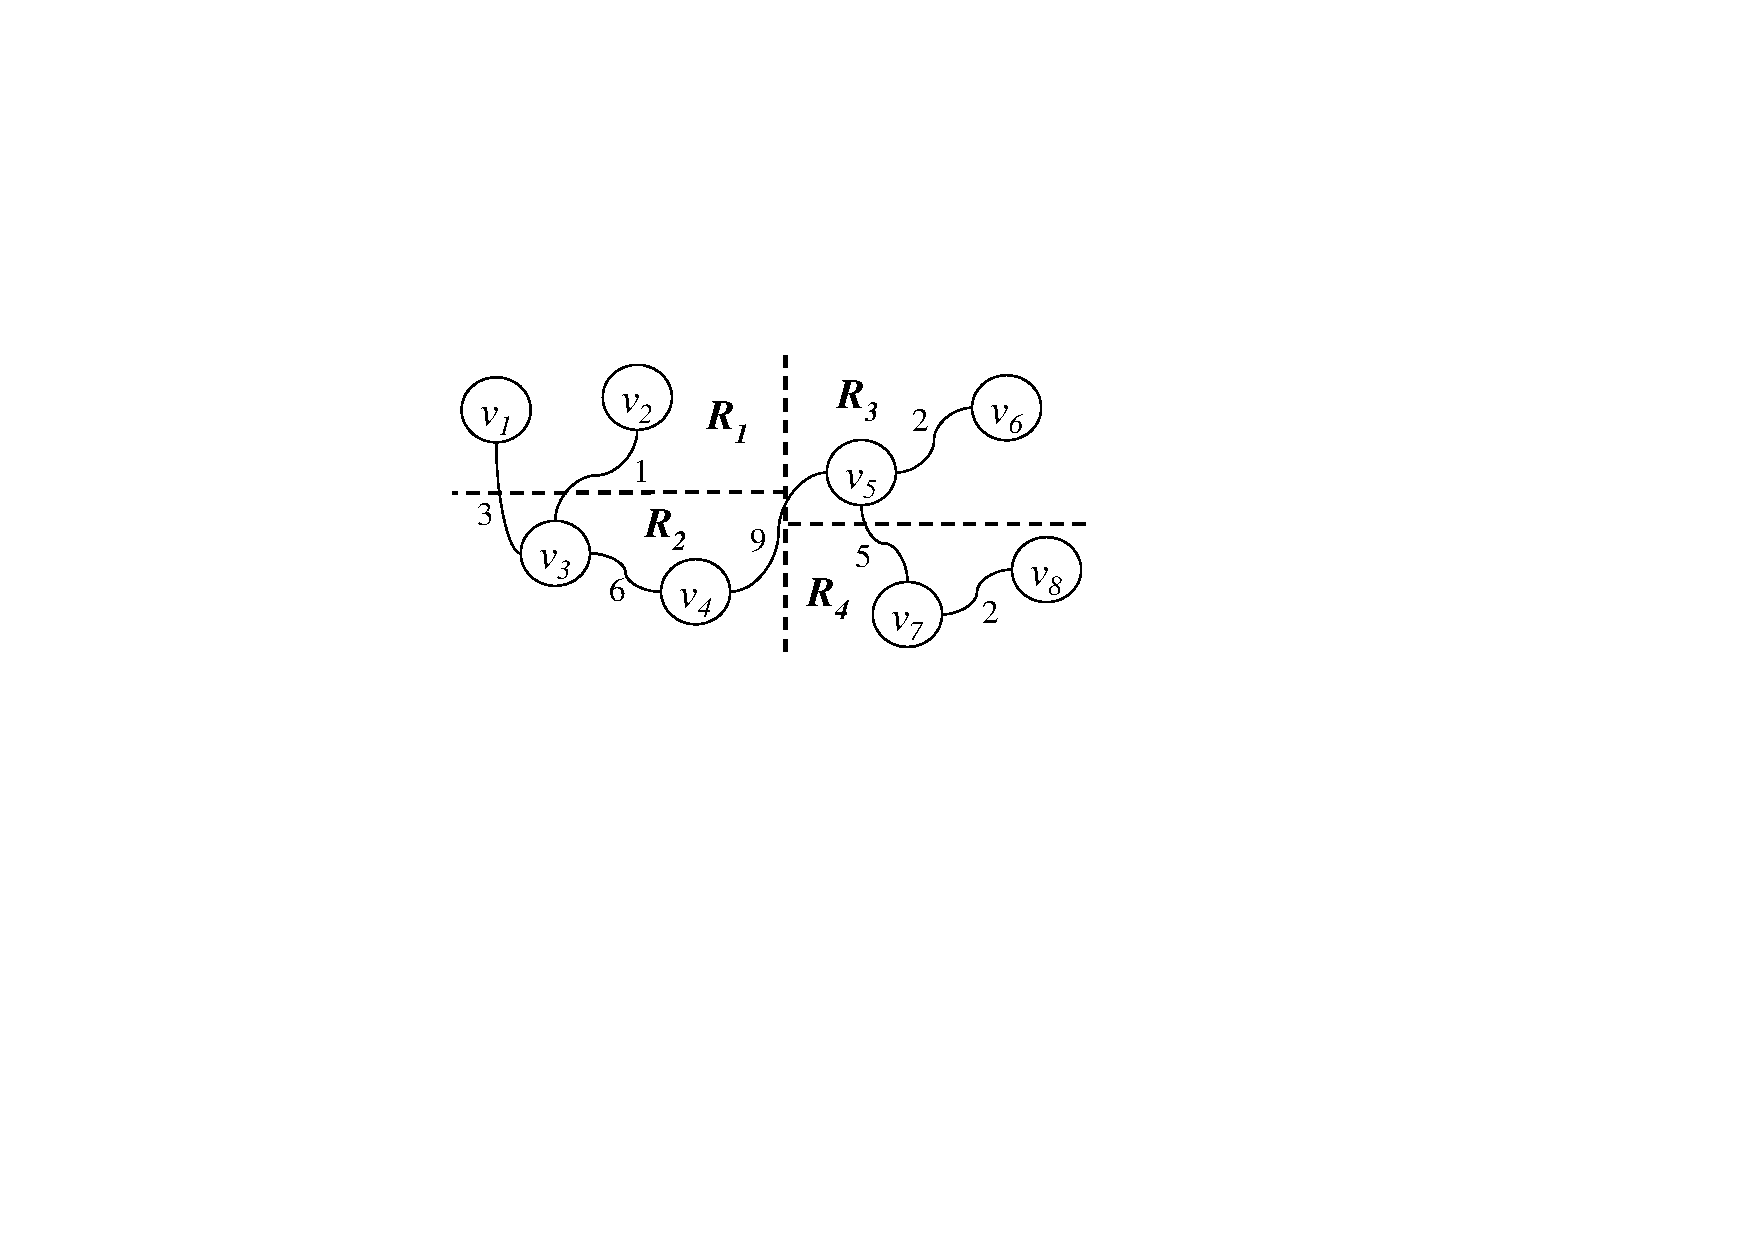
\includegraphics[width=0.68\columnwidth]{images/mappartition}} \\
& \\

	\begin{tabular}{|@{ }c@{ }|@{ }c@{ }c@{ }c@{ }c@{ }|}
	\hline \small
	\textbf{$\chi_{R_i,R_j}$}	& $R_1$		& $R_2$		& $R_3$		& $R_4$\\\hline
	$R_1$			& 0	& 1	& 2	& 1 \\ 
	$R_2$			& 1	& 0	& 3	& 1 \\ 
	$R_3$			& 2	& 3	& 0	& 0 \\ 
	$R_4$			& 1	& 1	& 0	& 0 \\ 
	\hline
	\end{tabular}
	\\
&
% \multicolumn{2}{c}{\includegraphics[width=0.75\columnwidth]{images/rxmap}}
  
\end{tabular}

\end{frame}




\subsection{Cost Estimation}
\begin{frame}[red] %hmm.. thought i could change colour here :S
\frametitle{SP Call Cost Estimation} 


\begin{columns}[b]
  \begin{column}{0.5\textwidth}
\begin{exampleblock}{Proxy Scenario}
$E_{s,t}(Proxy) = 1$
\end{exampleblock}

\begin{exampleblock}{Server Scenario}
Intuition: Longer query results incur higher cost.
\end{exampleblock}

$-$ Cost only estimated in server scenario\\
$-$ Estimation methods developed for Server scenario
  \end{column}
  \begin{column}{0.45\textwidth}

  \end{column}
\end{columns}


  \begin{picture}(0.0,0.0) 
     \put(160,30){  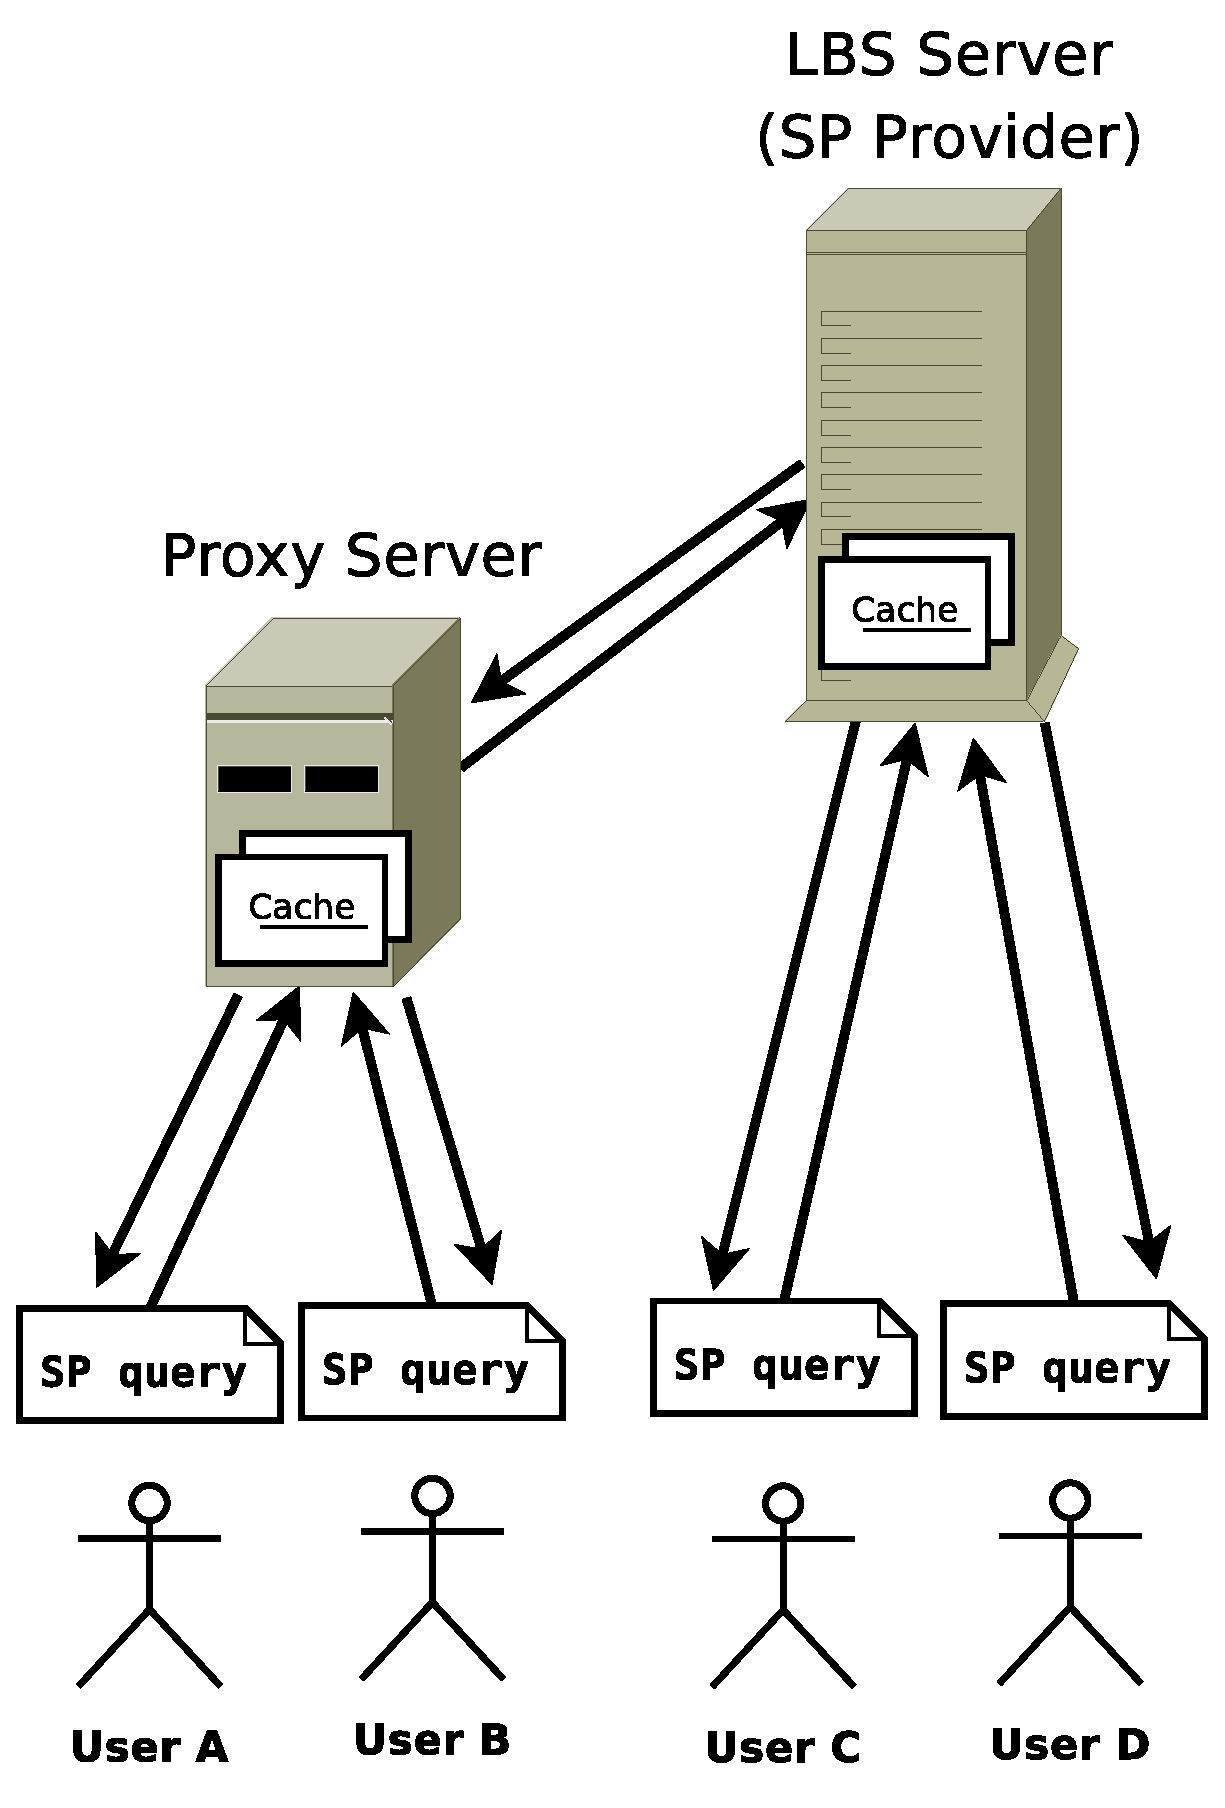
\includegraphics[width=0.5\textwidth]{images/scenario} }
  \end{picture}



% Two data structures:
% \begin{itemize}
%   \item Distance estimator, Landmark-based [Potamias et al. CIKM]
%   \item Expense histogram
% \end{itemize}
\end{frame}


\subsection{Benefit Model}



\begin{frame} %hmm.. thought i could change colour here :S
\frametitle{Incremental Benefit per size} 
  \begin{block}{Benefit formula}
    $\Delta\overline{\gamma}(P_{a,b}, \Psi) = \sum\limits_{P_{s,t} \in \mathfrak{U}(P_{a,b}) - \mathfrak{U}(\Psi)} \frac{\chi_{s,t} * E_{s,t}}{|P_{a,b}|}$
  \end{block}


\begin{itemize}
\item $P_{a,b}$: a shortest path 
\item $\Psi$: the cache 
\item $\mathfrak{U}(P_{a,b})$: all sub-paths of $P_{a,b}$. 
\item $\chi_{s,t}$ frequency of query $s$ to $t$. 
\item $E_{s,t}$: cost of calculating $P_{s,t}$
\end{itemize}

\end{frame}

% \begin{frame} %hmm.. thought i could change colour here :S
% % \frametitle{Benefit Model} 
% 
% \begin{columns}
%   \begin{column}{0.4\textwidth}
% From Query Log:
%   \begin{tabular}{|l|l|}
%     Shortest Path & Frequency \\\hline
%     $P_{3,6}$ & 3 \\
%     $P_{1,4}$ & 1 \\
%     $P_{1,6}$ & 1 \\
%   \end{tabular}
%   \end{column}
%   \begin{column}{0.1\textwidth}
%   \end{column}
%   \begin{column}[t]{0.6\textwidth}
% Cost Estimation:\\
%   \begin{tabular}{|l|l|}
%     Shortest Path & Cost \\\hline
%     $P_{3,6}$ & 3 \\
%     $P_{1,4}$ & 2 \\
%     $P_{1,6}$ & 4 \\
%   \end{tabular}
%   \end{column}
% \end{columns}
% 
% 
%     \includegraphics[width=0.4\textwidth]{images/rxmap} 
% 
%     \hspace{-2em}$\gamma(\Psi)=1*2+1*4+3*3=15$\\
% 
%   \begin{exampleblock}{$\gamma(P_{1,6}) + \gamma(P_{3,6}) \neq \gamma(\Psi)$}
% \hspace{0.7em} (15) \hspace{1.8em} (9)
%   \end{exampleblock}
% \end{frame}


\begin{frame}[shrink=5]  %hmm.. thought i could change colour here :S
\frametitle{Cache: SP Result Ranking} 

 Greedy algorithm


{\small
\begin{tabular}{@{}|c@{}|c@{}|@{}}
\hline
Timestamp & Query \\ \hline 
$T_1$ & $Q_{3,6}$ \\ \hline 
$T_2$ & $Q_{1,6}$ \\ \hline 
$T_3$ & $Q_{2,7}$ \\ \hline 
$T_4$ & $Q_{1,4}$ \\ \hline 
$T_5$ & $Q_{4,8}$ \\ \hline 
$T_6$ & $Q_{2,5}$ \\ \hline 
$T_7$ & $Q_{3,6}$ \\ \hline  
$T_8$ & $Q_{3,6}$ \\ \hline 
\end{tabular}
}


  \begin{picture}(0.0,0.0) 
     \put(90,5){  \includegraphics[width=0.7\textwidth]{images/rxmap} }
  \end{picture}



{\small
\begin{tabular}{|c||c|c|c|c|c|c||c|c|}\hline
    Round & \multicolumn{6}{c||}{Path} & \multicolumn{2}{@{ }c@{ }|}{Cache $\Psi$ }  \\ \cline{2-9}
             	& $P_{1,4}$ & $P_{1,6}$ & $P_{2,5}$ & $P_{2,7}$ & $P_{3,6}$ &  $P_{4,8}$ & Before &  After 	 	 \\\hline \hline
    1	&  1/3    & \zebox{\bf 5/5}	 & 1/4    & 2/5 &  3/4    & 1/4 &  empty    & $P_{1,6}$ \\\hline
    2	&      &  &     &  &     &  & $P_{1,6}$    & $P_{1,6}, {\bf ?}$  \\\hline
\end{tabular}
}
\end{frame}


\begin{frame}[shrink=5]  %hmm.. thought i could change colour here :S
\frametitle{Cache: SP Result Ranking - Incremental benefit} 


Incremental benefit calculation



{\small
\begin{tabular}{@{}|c@{}|c@{}|@{}}
\hline
Timestamp & Query \\ \hline 
$T_1$ & $Q_{3,6}$ \\ \hline 
$T_2$ & $Q_{1,6}$ \\ \hline 
$T_3$ & $Q_{2,7}$ \\ \hline 
$T_4$ & $Q_{1,4}$ \\ \hline 
$T_5$ & $Q_{4,8}$ \\ \hline 
$T_6$ & $Q_{2,5}$ \\ \hline 
$T_7$ & $Q_{3,6}$ \\ \hline  
$T_8$ & $Q_{3,6}$ \\ \hline 
\end{tabular}
}


  \begin{picture}(0.0,0.0) 
     \put(90,5){  \includegraphics[width=0.7\textwidth]{images/rxmap} }
  \end{picture}



{\small
\begin{tabular}{|c||c|c|c|c|c|c||c|c|}\hline
    Round & \multicolumn{6}{c||}{Path} & \multicolumn{2}{@{ }c@{ }|}{Cache $\Psi$ }  \\ \cline{2-9}
             	& $P_{1,4}$ & $P_{1,6}$ & $P_{2,5}$ & $P_{2,7}$ & $P_{3,6}$ &  $P_{4,8}$ & Before &  After 	 	 \\\hline \hline
    1	&  1/3    & \zebox{\bf 5/5}	 & 1/4    & 2/5 &  3/4    & 1/4 &  empty    & $P_{1,6}$ \\\hline
    2	&  0    & 0 &  1/4    & \zebox{\bf 2/5} &  0    & 1/4 & $P_{1,6}$    & $P_{1,6}, P_{2,7}$  \\\hline
\end{tabular}
}
\end{frame}


\subsection{Data Structure}
\begin{frame}[red] %hmm.. thought i could change colour here :S
\frametitle{Efficient Data Structure for the Cache} %Maybe a figure to easily explain the main point

\begin{itemize}
\item Lookup time grows with size cache 
\item Support return of full or partial cache items
\item Compact storage of shortest paths
\end{itemize}

\begin{figure}[hbt]
  \center %\small
  \begin{tabular}{@{}c@{}c@{ }c@{}}
    \begin{tabular}{c|l|}
        \cline{2-2}
        $\Psi_1$ & $v_1, v_3, v_4$ \\ \cline{2-2}
        $\Psi_2$ & $v_1, v_3, v_2$ \\ \cline{2-2}
        $\Psi_3$ & $v_2, v_3, v_4, v_5$ \\ \cline{2-2}
%        $\Psi_4$ & $v_3, v_4, v_5, v_6$ \\ \cline{2-2}
%        $\Psi_5$ & $v_3, v_4, v_5, v_7$ \\ \cline{2-2}
    \end{tabular}
    &
    \begin{tabular}{c|l|}
        \cline{2-2}
        $v_1$ & $\Psi_1, \Psi_2$ \\ \cline{2-2}
        $v_2$ & $\Psi_2, \Psi_3$ \\ \cline{2-2}
        $v_3$ & $\Psi_1, \Psi_2, \Psi_3$ \\ \cline{2-2}
        $v_4$ & $\Psi_1, \Psi_3$ \\ \cline{2-2}
        $v_5$ & $\Psi_3$ \\ \cline{2-2}
    \end{tabular}
  &
    \begin{tabular}{c}
    \\
    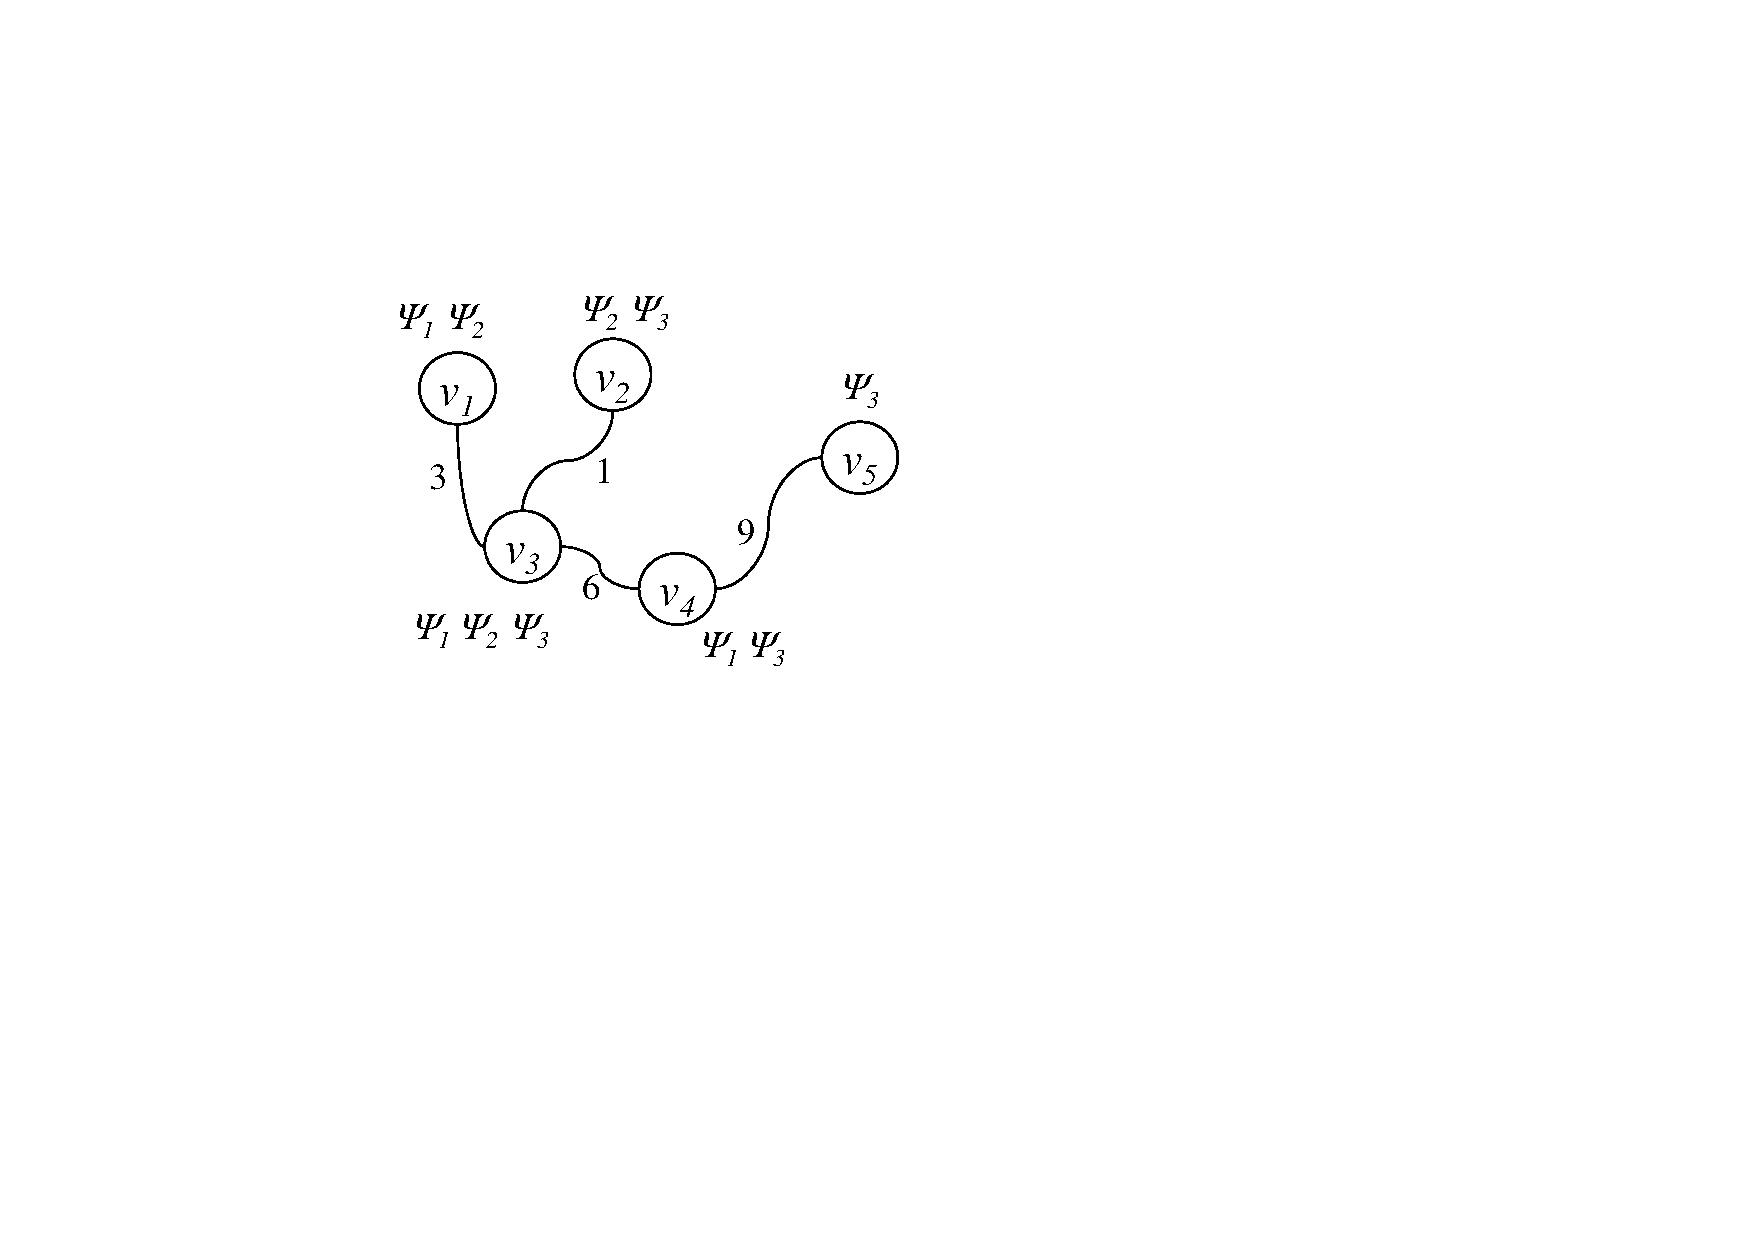
\includegraphics[width=0.4\columnwidth]{images/cachegraph}
    \end{tabular}
    \\
     Paths & \hspace{1.5em} Inverted List & \hspace{1.5em} Visualization
  \end{tabular}
\end{figure}

\end{frame}


\begin{frame}[shrink=10] %hmm.. thought i could change colour here :S
\frametitle{Efficient Data Structure for the Cache} %Maybe a figure to easily explain the main point

\begin{itemize}
\item Support efficient lookup and return of full or partial cache items\\
\item Compact storage of shortest paths
\end{itemize}
\makebox[\linewidth]{\parbox{14cm}{
\begin{figure}[hbt]
  \center \small \hspace{-2em}
  \begin{tabular}{@{}c@{}c@{ }c@{}}
    \begin{tabular}{c|l|}
	      \multicolumn{2}{c}{} \\\cline{2-2}
        $v_1$ & $v_3$ \\ \cline{2-2}
        $v_2$ & $v_3$ \\ \cline{2-2}
        $v_3$ & $v_1, v_2, v_4$ \\ \cline{2-2}
        $v_4$ & $v_3, v_5$ \\ \cline{2-2}
        $v_5$ & $v_4$ \\ \cline{2-2}
    \end{tabular}
   &
    \begin{tabular}{c|l|c|}
        \multicolumn{3}{c}{~~~~~~content~~~~parent} \\
        \cline{2-3}
        $v_1$ & $\Psi_1, \Psi_2$ & NIL \\ \cline{2-3}
        $v_2$ & $\cdots$ & $\cdots$ \\ \cline{2-3}
        $v_3$ & $\Psi_3$ & $v_1$ \\ \cline{2-3}
        $v_4$ & $\cdots$ & $\cdots$ \\ \cline{2-3}
        $v_5$ & $\cdots$ & $\cdots$ \\ \cline{2-3}
    \end{tabular}
  &
    \begin{tabular}{@{}c@{}}
    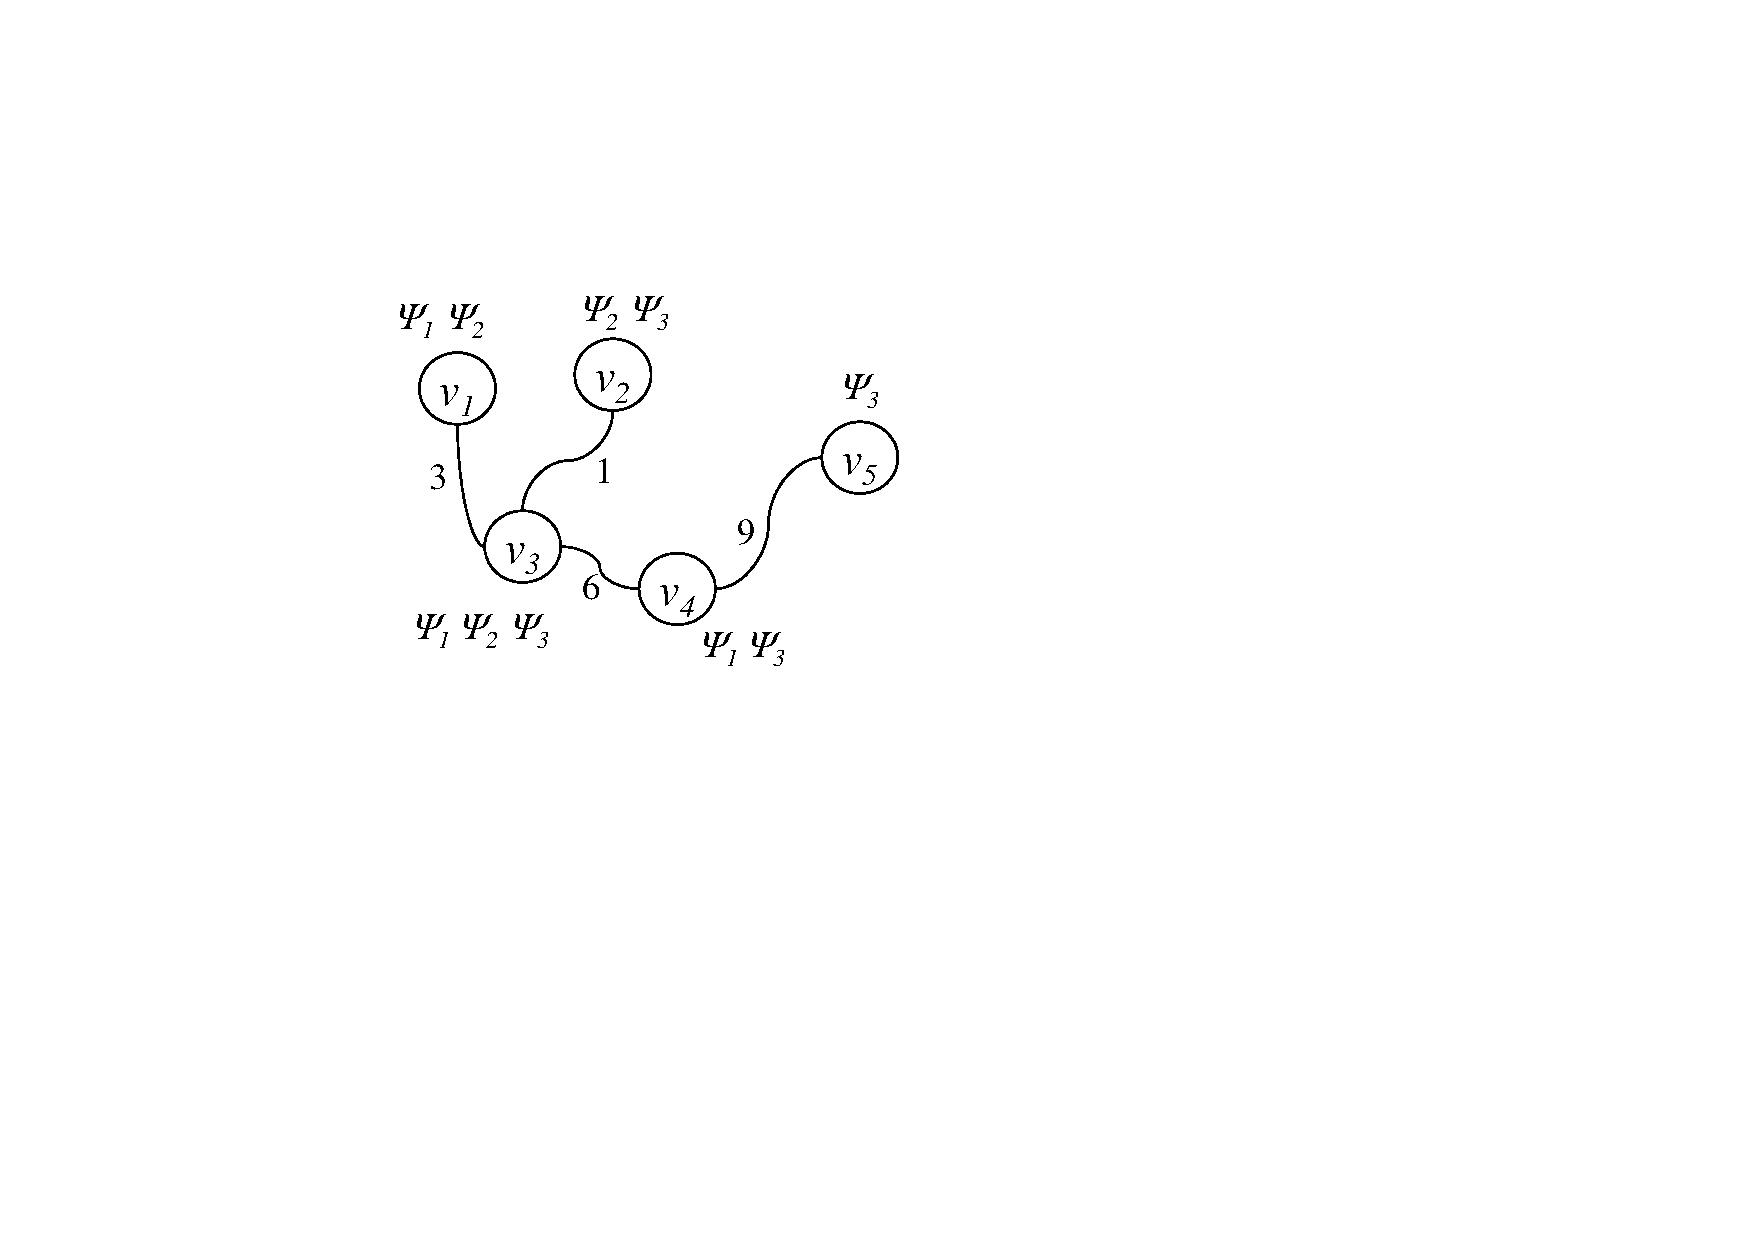
\includegraphics[width=0.45\columnwidth]{images/cachegraph}
    \end{tabular}
    \\
    %\hspace{1.5em}Inverted lists & 
    \hspace{1em}Graph representation &  \hspace{1.5em}Prefix compressed & Visualization
  \end{tabular}
\end{figure}
}}

\end{frame}
%
% \section{Algorithm}\label{sec:algorithm}

To clarify how we intend our approach to actually work we clarify concepts such as Road types, how protection schemes will be chosen, and how exactly we intend to apply the spatial and temporal anonymity of \tanonns. 

We will additionally present a set of algorithms to show how we intend our approach to handle the anonymization process.



\subsection{Applicability of Protection Schemes}

When users choose a classification for a \poi the system will attempt to automatically make some choices with regards to what the best way to anonymize that \poins. These choices are presented in table~\ref{tab:poitype} where it is shown which protection scheme(s) (Sec.~\ref{subsec:schemes}) is applicable for each classification. The trajectories will be sorted based on the classification of the \poi specifying sensitivity of its edges (possibly one trajectory will be have sub-trajectories sorted into multiple groups).

The first classification: "Public Service Point" is straight forward, the \ac{AS} scheme will always be chosen as the classification covers hospitals, clinics and the like, and thus always will be sensitive. 

The second classification is "House" which covers homes or institutions (e.g. a kindergarden). These will either only be sensitive on a one time basis i.e. use the \ac{RS} scheme, or only be sensitive at specific times when arriving or departing, leading to the \ac{ASTI} scheme.

\begin{table}[Htb]
\center
\begin{tabular}{|l|l|l|}
\hline
\bf Classification	& \bf Scheme \\\hline		
Public Service Point	& \ac{AS} \\\hline
House			& \ac{ASTI}, \ac{RS} \\\hline
Route w. endpoints	& \ac{AS}, \ac{ASTI}, \ac{RS}  \\\hline
Route w/o endpoints	& \ac{AS}, \ac{ASTI}, \ac{RS}  \\\hline

\end{tabular}
\caption{Applicability of protection schemes and types for different \poisns} 
\label{tab:poitype}
\end{table}



\subsection{Road Types} \label{subsec:roadtypes}

\rt was first mentioned in section \ref{subsec:probdef} when we defined road segment as having a road type(\rt) associated with it. A $\rt \in \mathbb{N}$ is a hierarchy imposed in the edges of a road network to express how busy or important one road is compared to another road (e.g. highway > paved road > dirt road). \rt is used when the system needs to alter a trajectory by adding or removing edges in a trajectory (Sec. \ref{subsec:addremoveEdges}). 
The algorithm aims to preserve the truth of the data so when the anonymized data is later analyzed it will still represent the same traffic tendencies. \rts are used in the calculation of Road Difference, where a difference in roadtypes of two edges will impose a penalty when calculating weather it is okay to take add a detour on a local road i.e. it is okay via another nearby local road, but it is not okay to make the detour on the highway. The rationale behind this is that people {\it choose} to either take the highway or some smaller road when going from point A to B. Adding highway edges to a trajectory originally only containing smaller \rts , like e.g. a dirt road, would be a misrepresentation of the original data in the anonymized dataset. Wether it is okay to add/delete an edge in a trajectory depends on equation~\ref{eq:ediff} where the Road Difference is used as a penalty. Road Difference is defined as:

\begin{deff}[Road Difference]
\label{def:roaddiff}
Given two edges \(e_1, e_2\) the Road difference is $| e_{1_{RT}} - e_{2_{RT}} |$
\end{deff}


\subsection{Methods of Trajectory Obfuscation}

In this section we present the two methods we will be using to archive \tanonns: Trajectory Alignment and Timestamp Modification.

When trying to protect a the sensitive edges, covered by a \poins, in a trajectory one way is to create an alternative route from two points (Fig.~\ref{fig:altRoute},~Alt), avoiding the sensitive edges all together. Another way is to align trajectories to be alike which is the way we will handle the spatial aspect of \tanon of making \(t\) sub-trajectories indistinguishable. This is described below in \ref{subsec:addremoveEdges}. To handle the temporal aspect of \tanon we do timestamp modification as explained in section~\ref{subsec:timeMod}


%The first is regarding the scenario where a \poi only has one single long road going too and from it. If this happens it will make no sense to e.g. just remove five edges before/after the \poi since it will be clear that the original trajectory could only have gone though the POI where we removed the edges.


\subsubsection{Trajectory Alignment}\label{subsec:addremoveEdges}

We want to add and remove edges in trajectories to make them look as similar as possible and thereby archiving a degree of spatial anonymity. We do not want to destroy the traffic pattern in the original dataset so only trajectories where adding or removing edges result in a deviation from the original trajectory below a system parameter $\mathbf{D}$ will be considered when trying to fulfill users privacy requirements.

Since two trajectories may not be the same length, or have the same number of edges over the same distance we need to first align them before comparing edges and determining how similar two trajectories may be. 
To align two trajectories, T1, T2, we first find the shortest path from all vertices in T1 to vertices in T2 (See. Fig.~\ref{fig:edgeAlign}A). If any vertices in T2 has not been reached (e.g. Fig.~\ref{fig:edgeAlign}A $t_{25}, t_{26}$) we will find the shortest path from these to vertices in T1. 
When choosing which edges to compare we always use T1 as our starting point. This gives us 2 cases (Fig.~\ref{fig:edgeAlign}B (A\&B)) when choosing which edge in T2 to compare with. 

Equation~\ref{eq:cEdge} takes two vertices from T1 (a,b) and two from T2 (c,d). It finds the shortest total distance of two pair, each consisting of one vertice from each trajectory, and it returns the two pairs with collective shortest euclidean distance.

In case A we have edge \(e_{11}\) with both vertices ($t_{11},t_{12}$) having a shortest path to the same vertice, $t_{21}$, in T2. Since $t_{21}$ only have one outgoing edge we will compare \(e_{11}\) and \(e_{21}\).
In case B the end vertices of $e_{13}$ each have a different closest vertice in T2, so to find the closest edge in T2 we find the smallest total distance from $(t_{13},t_{14})$ to any pair of vertices in T2 laying between \(t_{22}\) and \(t_{24}\), both vertices included. To find the closest edge to $e_{13}$ in T2 we use equation~\ref{eq:cEdge} to calculate: \(Min\left(N_{edge}(t_{13},t_{14},t_{22},t_{23}),N_{edge}(t_{13},t_{14},t_{23},t_{24})\right)\) and return the two pairs of end vertices having the smallest total distance.

Once we have determined which edges in T1 to compare with in T2, do the same for any edges in T2 which have yet to be matched with an edge in T1. This leads to edges in one trajectory possibly being the closest edge to several edges in another trajectory. Equation \ref{eq:dEdge} finds the total minimum distance between the two pairs of end vertices using the vertices of the input edges as arguments for \(N_{edges}\).

When we have determined which edges to compare we calculate the difference between them using equation~\ref{eq:ediff} where \(d(e_{1}, e_{2}) \) is divided by two to get the mean distance between $e_1,e_2$ and  \(|e_{1_{RT}} - e_{2_{RT}}|\) is the Road Difference which adds a penalty based on any difference in roadtypes of the two edges compared.
When calculating the difference between two trajectories, or sub-trajectories, we use equation~\ref{eq:tdiff} 


\begin{figure}	
  \center
  \begin{tabular}{c}
	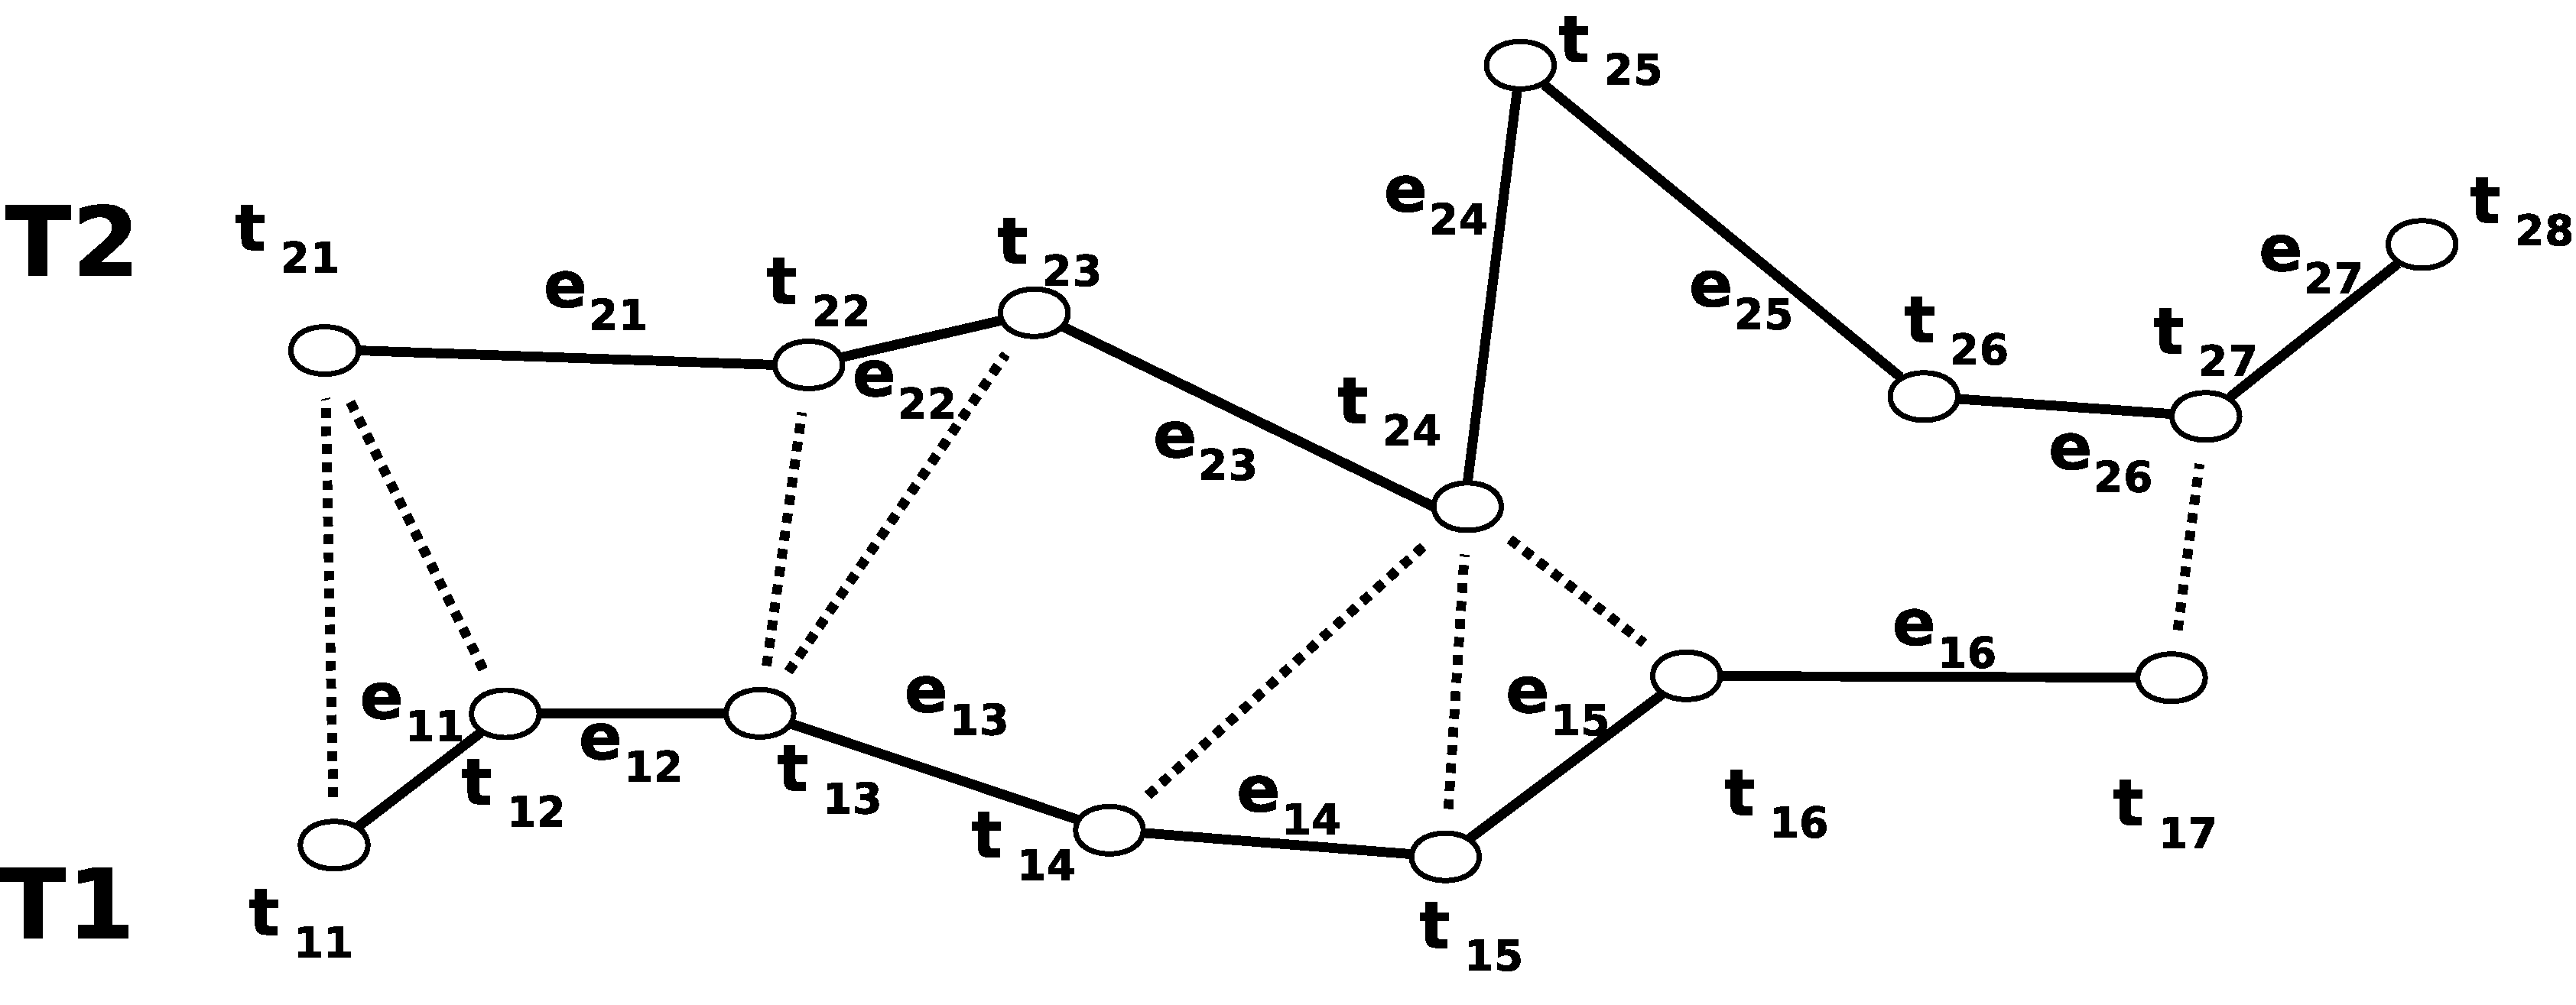
\includegraphics[width=0.5\textwidth]{figures/edgeAlignment2} \\\hline
	{\bf(A)} \\
	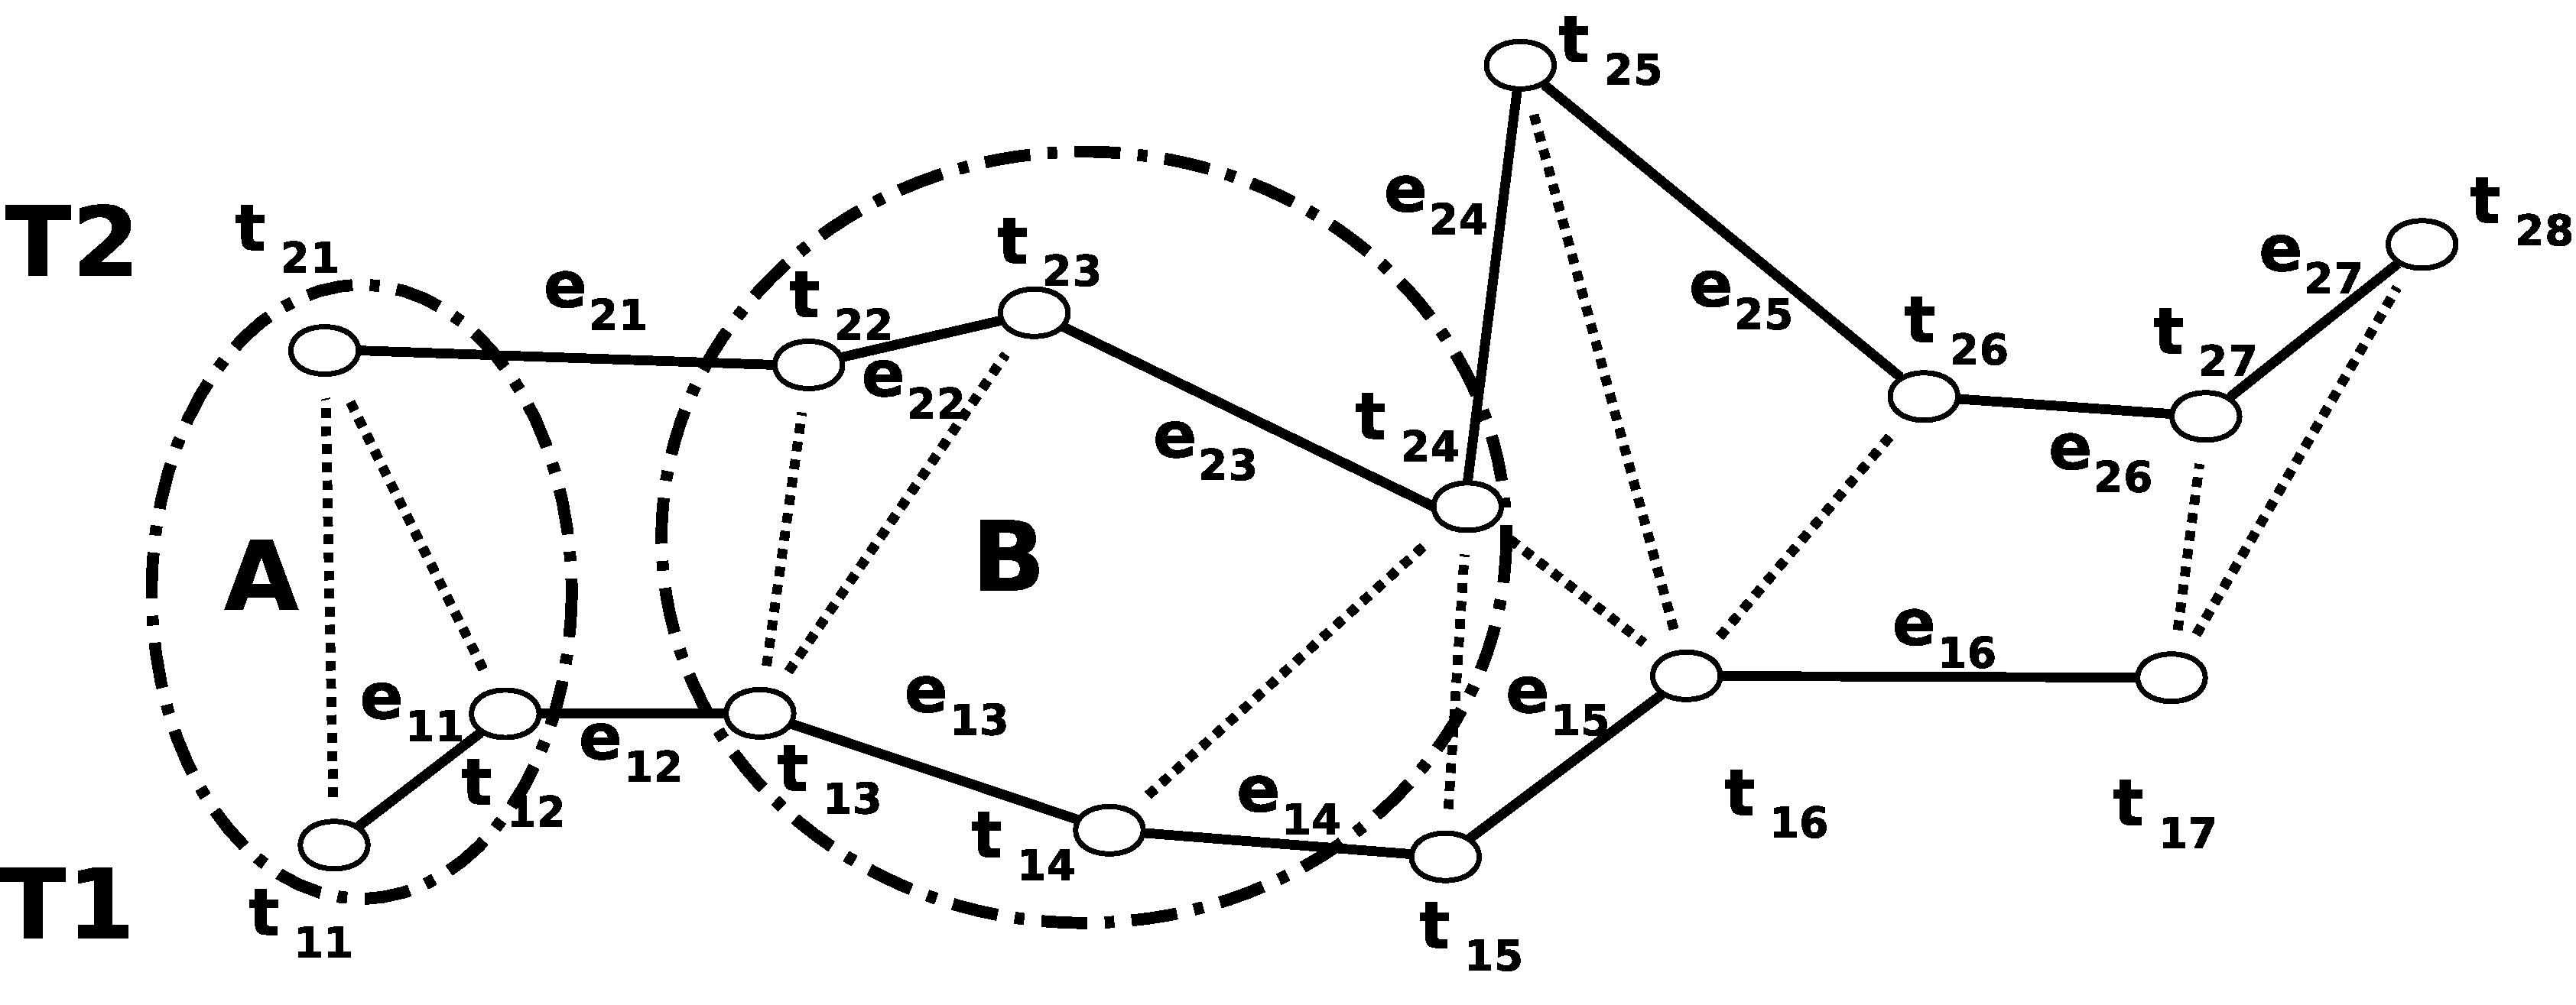
\includegraphics[width=0.5\textwidth]{figures/edgeAlignment3} \\\hline
	{\bf(B)}
  \end{tabular}
  \caption{Edge Alignment when comparing two trajectories}
  \label{fig:edgeAlign}
\end{figure}

\begin{equation}\label{eq:cEdge}
N_{edge}(a,b,c,d) = Min\left(| ac | + | bd |, | ad | +| bc | \right)
\end{equation} 

\begin{equation}\label{eq:dEdge}
d(e_{1}, e_{2}) = | N_{edge}(e_1.v_s, e_1.v_e, e_2.v_s, e_2.v_e) |
\end{equation} 

\begin{equation}\label{eq:ediff}
e_{diff}(e_1,e_2) = \left( \frac{d\left(e_{1}, e_{2}\right)}{2} \right) * (1+|e_{1_{RT}} - e_{2_{RT}}|)
\end{equation}


\begin{equation}\label{eq:tdiff}
\;t_{diff}(t_1,t_2) = \frac{\sum_{\substack{k=1}}^m e_{diff}(t_1.e_k, t_2.e_k)}{m}
\end{equation}



% \begin{equation}\label{eq:rtlimit}
%  \sum_{m=0}^n (|e_{1_m} - e_{2_m}| + (RE_{Before_m} +  RE_{After_m}))
% \end{equation}


\begin{figure}	
\center
	  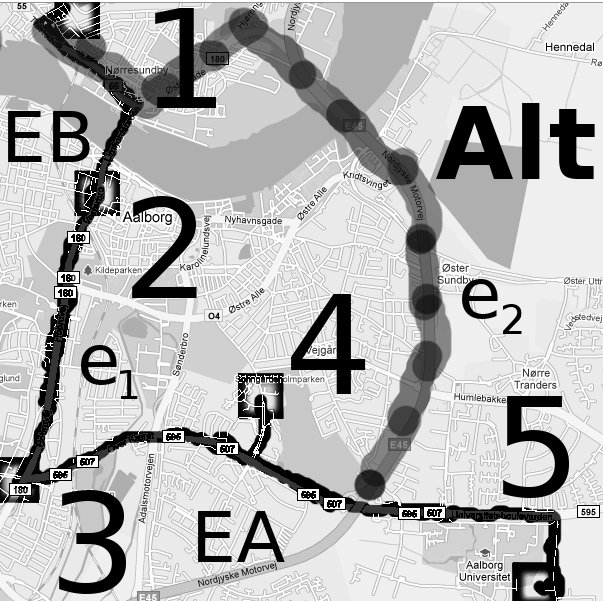
\includegraphics[width=0.2\textwidth]{figures/map2.jpeg}
       \caption{Alternative route}
  \label{fig:altRoute}
\end{figure}


\subsubsection{Timestamp Modification} \label{subsec:timeMod}

% 3 cases:
% 1. connect two trajectories in the \poi, making it seem as one person who never stopped
% 2. redistribute time across edges in the trajectory, making it seem like the user never stopped at the sensitive \poi
% 3. both do detour (in case hospital or other \poi is a small way off a larger road, then just cut away the small detour and patch up the trajectory.

As described in section \ref{subsec:protectiontypes}, when trying to protect a location which is on, or very near, a major road, one possible way of protecting the user is to simply make it look like the user never stopped and just drove right by the location. Figure~\ref{fig:adjustTrajec}A shows on the left side a sample trajectory with start-/end-time for each edge plus time not moving while the user has stopped at the hospital (here assumed to be defined as temporally sensitive). The graph on the right side of figure~\ref{fig:adjustTrajec} shows the distance the user has moved on the vertical axis and the time spent travelling on the horizontal axis. It can clearly be seen on the line for "Not Time adjusted (A)" that the user stops for an hour.

Figure~\ref{fig:adjustTrajec}B shows how the visit to the hospital can be removed simply by redistributing the time spent at the hospital onto the remaining edges on the trajectory, keeping in mind any limitations imposed by traffic or \rt (e.g. speed limits or road conditions). In the graph of figure~\ref{fig:adjustTrajec}, looking at the line for "Time adjusted (B)", it it now looks like the user just drove the entire length of the trajectory without stopping (in this case also at a fairly consistent speed).
The challenge is making sure that the travel times on the individual road-edges is still plausible after modifying the start-/end-times of some or all the road-edges. It can be insured using information about speed limits and average speeds the \rt (Sec.~\ref{subsec:roadtypes}) of the edges in the trajectory. In the example from figure~\ref{fig:adjustTrajec} the start and end times of the trajectory as whole has not been modified, but this is of cause an option but not described further in the algorithm. Adjusting the start and end times of a full trajectory allows for greater flexibility in case it is otherwise impossible to ensure a trajectory is destitute of all information relating to a stop at a sensitive location.


\begin{figure}	
       \center
       \begin{tabular}{cc}
		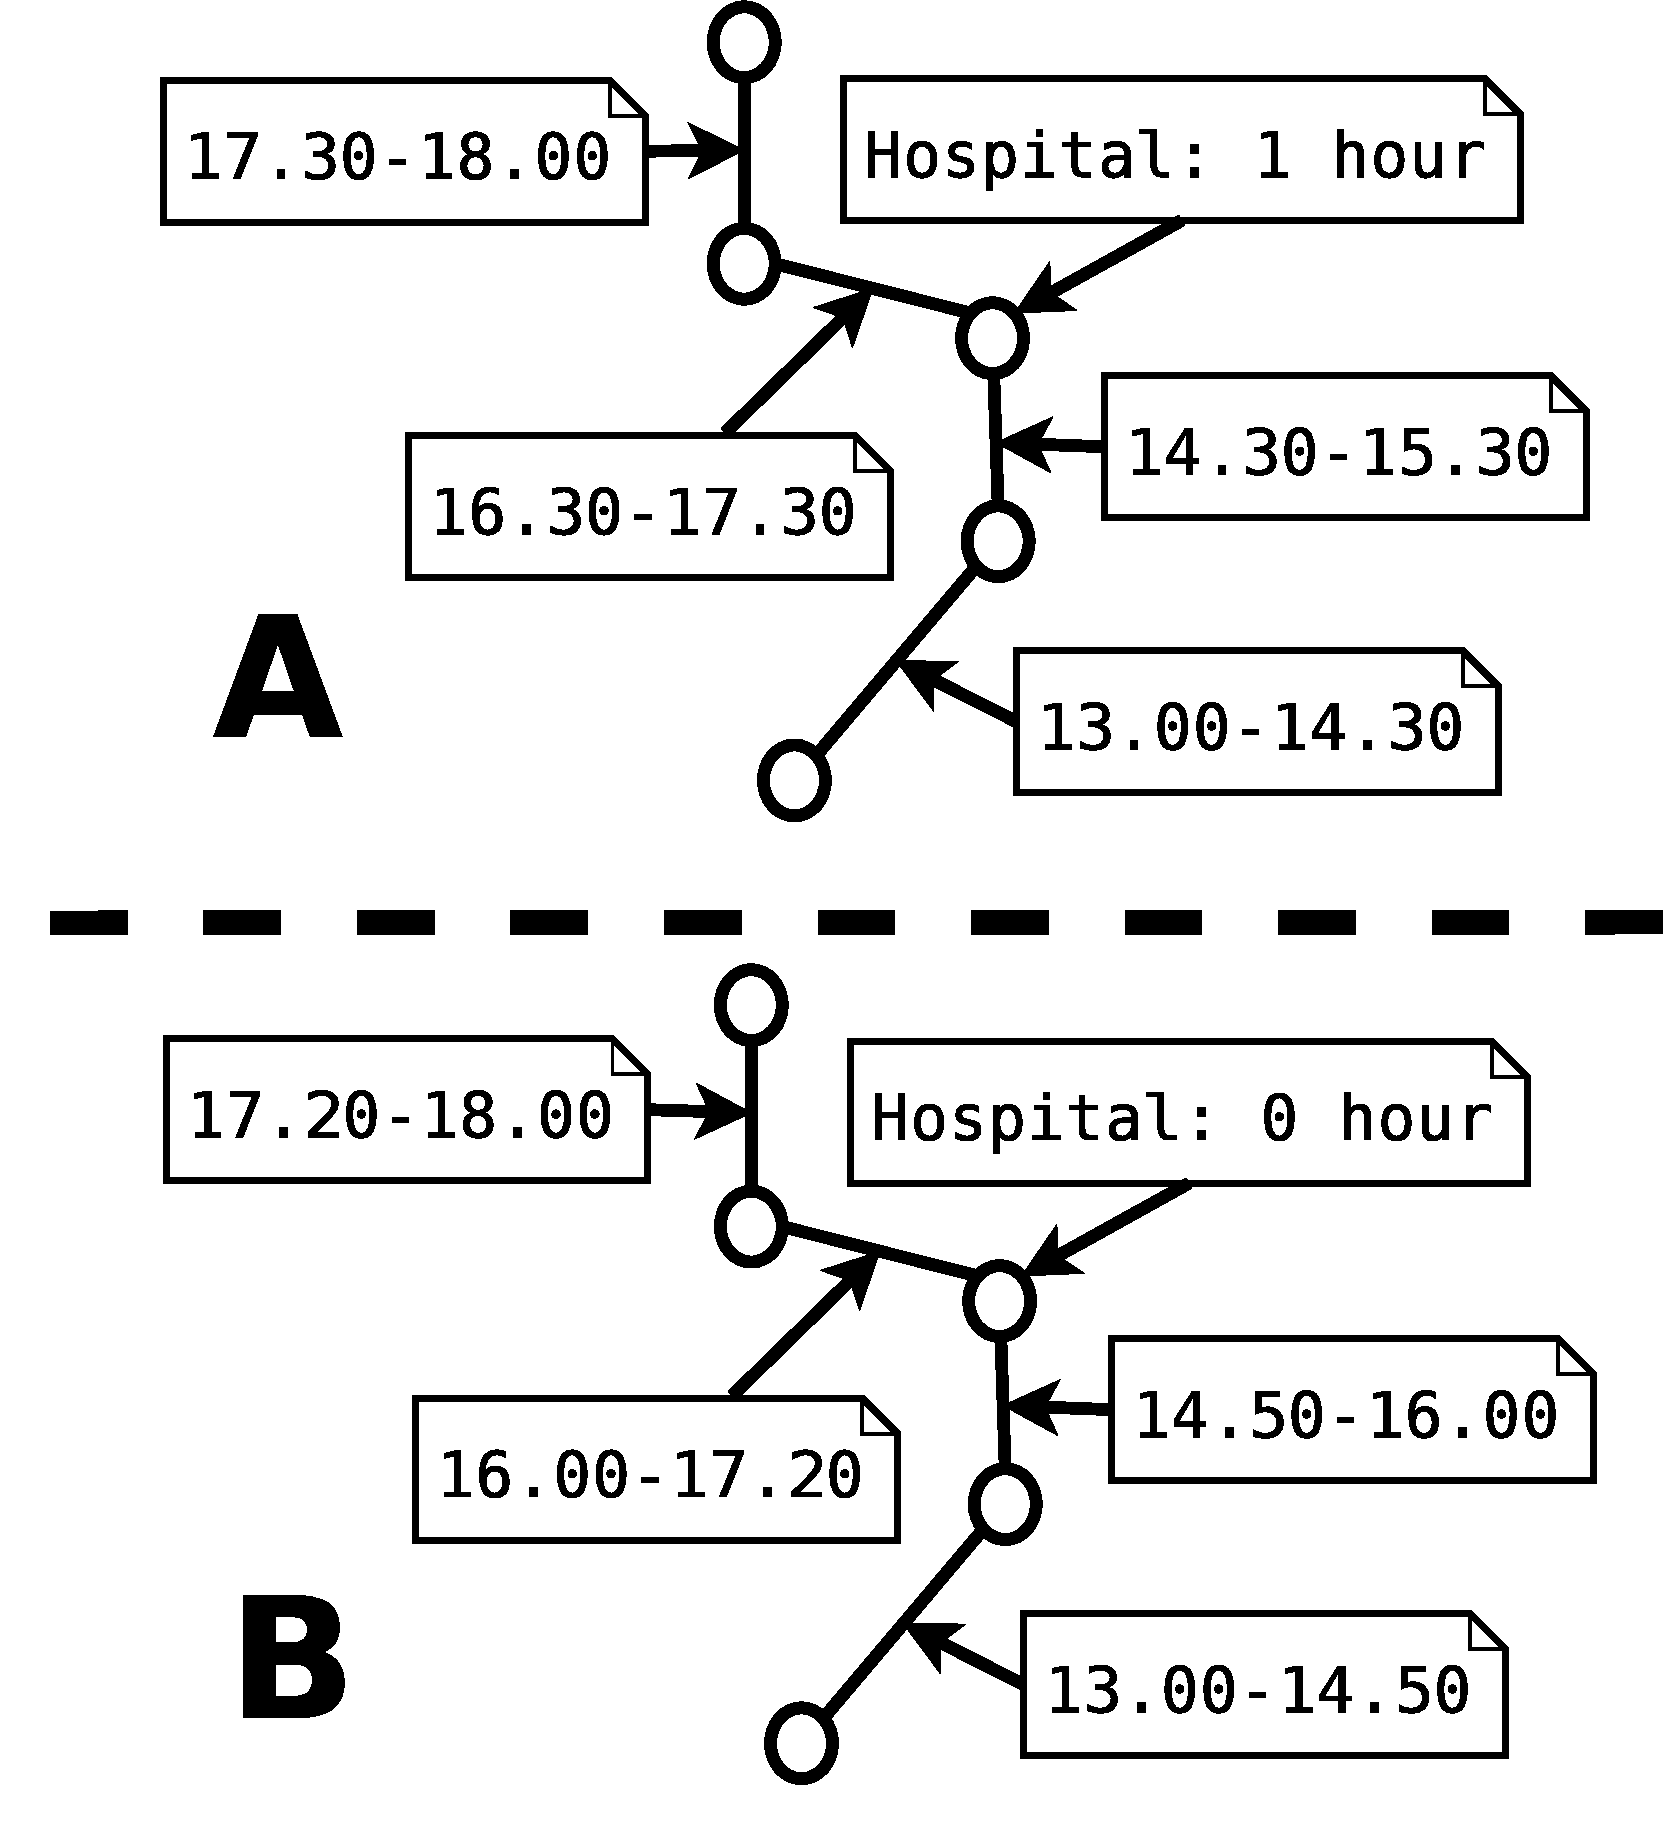
\includegraphics[width=0.20\textwidth]{figures/trajecAdjustTime.pdf} &
		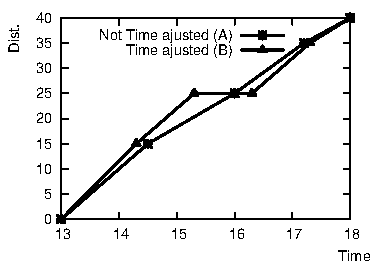
\includegraphics[width=0.25\textwidth]{figures/trajecAdjustTimeGraph.pdf} \\
	\end{tabular}
       \caption{Removal of visit to a hospital by distribution of time onto the road-segments of trajectory.}
  \label{fig:adjustTrajec}
\end{figure}



\subsection{Algorithm}

The algorithm consist of 5 parts, algorithm \ref{alg:overall} is the "master" algorithm which gives a good idea of the control flow in the algorithm, and 4 supporting algorithms, each handling a clearly defined step in algorithm \ref{alg:overall}. In most of the algorithms we work with a 4-tuple: $(t, t_{se}, d_{t}, d_{s})$ consisting of a trajectory, the set of edges in \(t\) defined as sensitive by a \poi and the temporal and spatial sensitivity values from the same \poins. The while loop in algorithm \ref{alg:overall} functions as the main control loop, only ending when there are no more unanonymized sub-trajectories left, i.e. trajectories which have some their edges covered by a \poi and which have not yet been included in $anonData$.
The best understanding of the algorithms will be archived by reading them in the numerical order they are presented, as each algorithm, except 1 \& 5, takes the output of the previous algorithm, modifies the data and returns the modified data.

The algorithms presented has a number of limitations introduced for readability and which should not interfere with the understanding of the how the approach works. First it is assumed that there is only one privacy profile per user, second it is assumed that each trajectory is only covered, or partly covered, by a single \poins. Third it is implicitly assumed that the given set of \pois and the trajectories they cover will "fit" according to their spatial and temporal sensitivities in each 4-tuple, such that after termination of the control loop in algorithm~\ref{alg:overall} no edge of any trajectory has been used twice.


\begin{algorithm}[H!bt]
\dontprintsemicolon
\SetVline

\SetKwInOut{Input}{input}\SetKwInOut{Output}{output}\SetKw{Return}{return}

\Input
{

	$G(V,E)$: Graph representation of Map \;
	$\Psi$: The cache \;
	$\mathcal{B}$: Cache budget \;
	
}
\vspace{0.7em}
\tcp{\emph{H Contains the utility score of all possible \spaths in $\mathbf{G(V,E)}$. The \spath is the value $v$ and the utility is the key $k$, $(k, v)$. The heap is sorted on the key.}}
H Initialize Max-Heap \;

\tcp{\emph{Initialially fill H}}

\ForAll{$\spath_{s,t} | s \in V, t \in V, s \neq t$} 
{
    H.push(S$(\chi, \spath_{s,t}, \Psi), \spath_{s,t}$) \;
}


\tcp{\emph{Fill cache}}
\While{$| \Psi | \leq \mathcal{B}$ AND $\spath_{ms}.k \neq 0$ OR $| H | > 0$}
{
	\tcp{\emph{Assign (utility,\spath) pair with the highest utility to $\spath_{ms}$}}
	$ \langle  key_{max},  SP_{max} \rangle \leftarrow$ H.pop() \; 
	\tcp{\emph{Update utility, as previous \spath insertion has changed it}}
	$key_{max} = S(\chi, \spath_{max}, \Psi)$
	\tcp{\emph{H.TopKey() looks at the top (k,v) pair without removing it from the heap}}
	\If{$key_{max} \geq H.TopKey$} 	
	{
	    \If{$( \mathcal{B} - | \Psi | ) \geq | \spath_{max} |$}
	    {
		$\Psi.insert(\spath_{max})$\;
	    }
	}
	\Else
	{
	    H.push(S$(\chi, \spath_{max}, \Psi), \spath_{max}$) \;
	}
}

\caption{\salgons($G(V,E), \Psi, \mathcal{B}$)}
\label{alg:greedy}
\end{algorithm}

The input to algorithm~\ref{alg:overall} contains all the concepts and parameters introduced in section~\ref{sec:problemdef} and \ref{sec:contribution} and it works as the main control loop, calling subsequent algorithms to anonymize sensitive edges in the set of trajectories \(\mathbf{T}\). The dataflow is such that each call to any of the four other algorithms provide a transformation on the input such that the output is can be used as the input for the next algorithm called.
The main while loop starts by choosing \(\alpha\), a tuple with trajectory containing a number of high sensitivity edges according to a \poi and calls the remaining algorithms on the basis of the chosen \(\alpha\). To choose \(\alpha\) the algorithm will handle the \poi types in the order given by table~\ref{tab:poiclass1} from top to bottom. \pois in each class will also be sorted according to their sensitivity values. The point in doing the \pois in order is that we want to ensure that all \poi are anonymized up to the highest level specified by a user with the least amount of work e.g. given two identical trajectories, one with sensitive endpoints and one without, it is important to choose the one with sensitive endpoints first as it is harder to anonymize and we therefor want to have as many candidates as possible to help anonymize that trajectory first.

The main loop ends when the privacy requirements of all \poi have been covered by some trajectories and ${\bf Choose\_\alpha}$ therefor can no longer find new tuples.
At the end of the main control loop all edges which has not been involved in the anonymization process is added to the anonymized dataset to have a complete dataset after anonymization.



\begin{algorithm}[H!bt]
\dontprintsemicolon
\SetVline

\SetKwInOut{Input}{input}\SetKwInOut{Output}{output}\SetKw{Return}{return}



\Input{
	$\mathbf{\spath_{s,t}}$: A \spath.\;
}

\Output{
	An integer representing the score
}



 \funcc{Score}{\spath_{s,t}}
{
	\textbf{H}.push($S(\chi, SP_{s,t}, \Psi), SP_{s,t}$) \;
% 	\ForEach{edge $e \in \alpha.t$}
% 	{
% 		\ForEach {$psr \in PS$ }
% 		{
% 			\If{$e \in psr.p_{edges}$}
% 			{
% 				${\poins}cand \leftarrow {\poins}cand \cup psr$\;
% 			}
% 		} 
% 	}
}

\caption{Score() function using statistics}
\label{alg:score}
\end{algorithm}

Algorithm~\ref{alg:findCan} finds the set of \poi which cover edges in \(\alpha.t_{se}\). The \poi set is needed to identify the set of trajectories which have edges with sensitivity values similar to \(\alpha\) in algorithm~\ref{alg:calcCan}. 

\begin{figure}	
       \center
	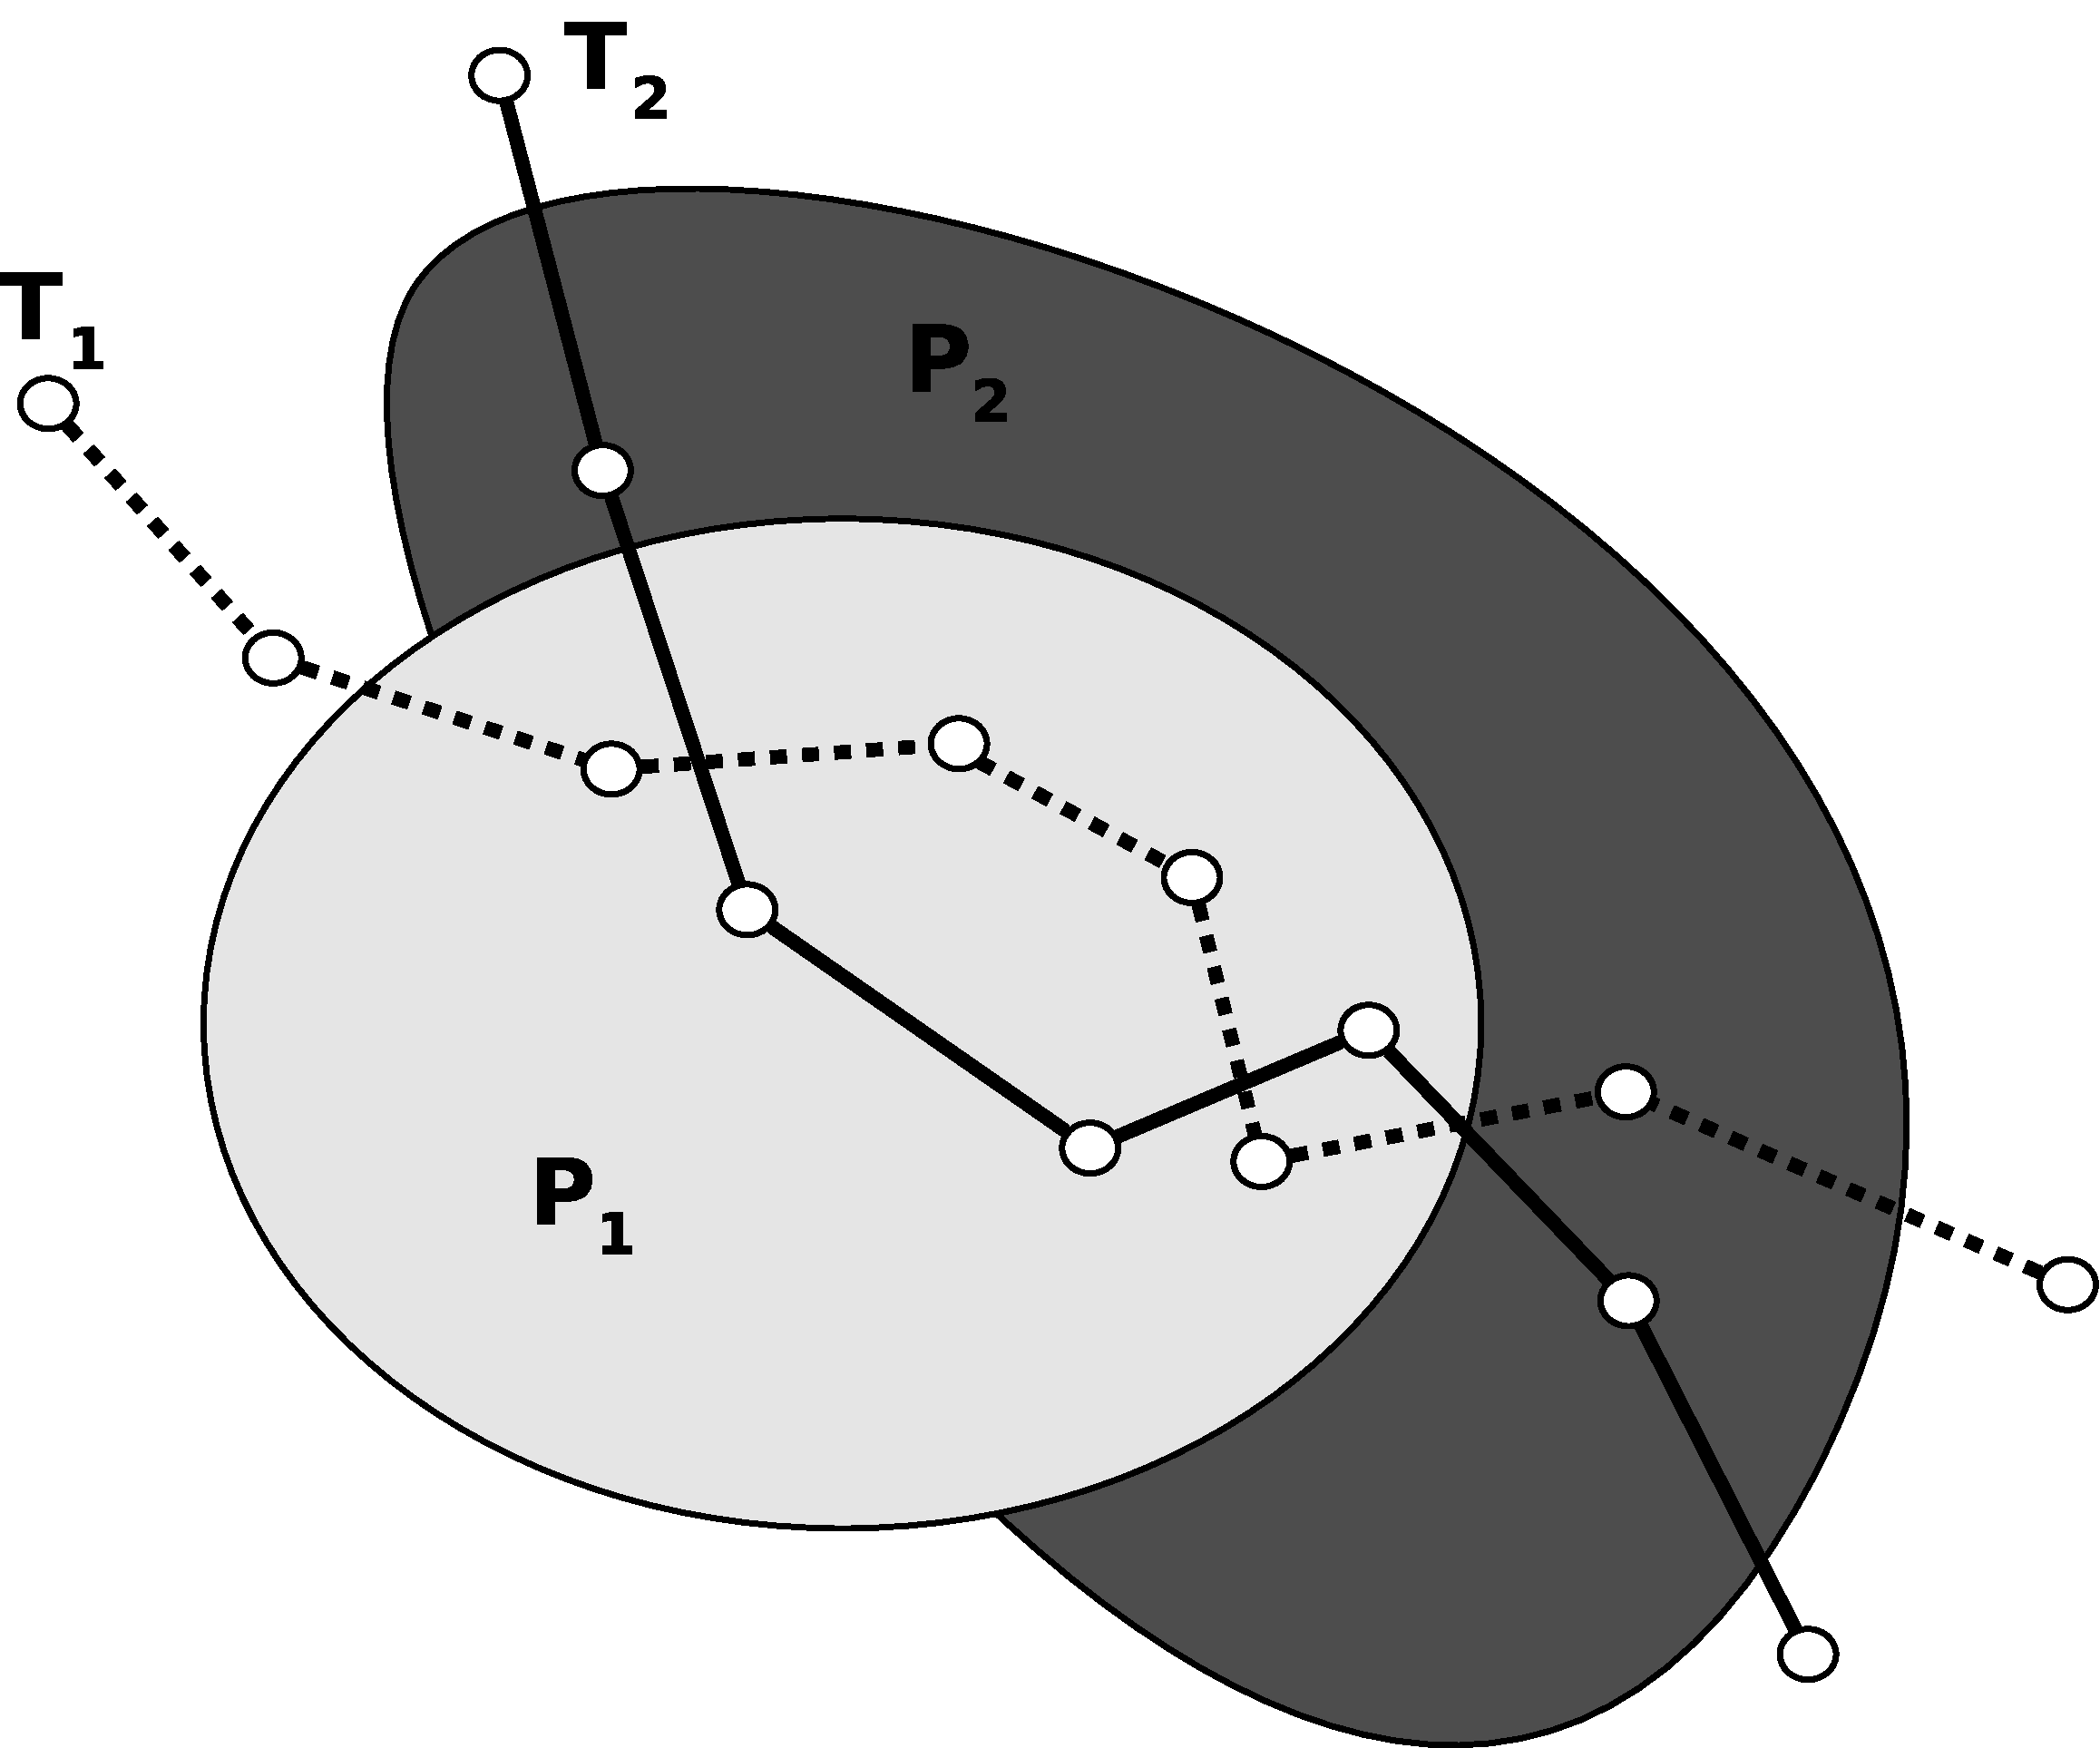
\includegraphics[width=0.40\textwidth]{figures/poiIntersect.pdf} 
       \caption{Two intersecting \poisns. $P_2$ covering all of $T_2$ edges, $P_1$ only covering some of $T_1$ edges. some edges in $T_1$ \& $T_2$ is covered by both \poins.}
  \label{fig:poiOverlap}
\end{figure}



\begin{algorithm}%[H!bt]

\dontprintsemicolon
\SetVline

\SetKwInOut{Input}{input}\SetKwInOut{Output}{output}\SetKw{Return}{return}


\Input{	$\mathbf{T}:$ The set of trajectories. \;

	\(t \in tCand:\) a tuple \((t, t_{se},t.d_t,t.d_s)\)

	$D \in \mathbb{R}$: Tolerance for how much a modified trajectory is allowed to diveate from original trajectory. \;

	$n \in \mathbb{N}$: Granularity of the road difference calculations. \;

	$\alpha$: a tuple $(t, t_{se}, d_{t}, d_{s})$  used as a base for anonymization.\;
}
\Output{

	$calcCand$: set containing calculated alternative trajectories along with their spatial and temporal sensitivity\;
}


\funcc{CalcAlt}{\alpha, t, D, n}
{
	$dLimit \leftarrow 0, diff \leftarrow 0, fail \leftarrow 0$ \;
	$j \leftarrow 1$ \;
	\(calcCand \leftarrow \emptyset\) \;


	$tmpT \leftarrow t.t \setminus \alpha.t$ \tcp{\emph{Ordered set}} \;
	

 	\While{$dLimit \leq D \wedge tmpT \backslash \alpha \neq \emptyset \wedge fail < 2$}
 	{
		%From the shared edges between $\alpha.t$ and $t.t$ choose edges alternating at each end of the shared edges.

		Choose edges alternating at each end of $tmpT$

		edge $e_1 \leftarrow \alpha.t[j]$ \;
		edge $e_2 \leftarrow {\bf closestEdge}(\alpha.t[j], t)$ \;

		\If{$\frac{e_{diff}(e_1,e_2,n) + diff}{j} \leq D$}
		{
			$diff \leftarrow e_{diff}(e_1,e_2,n) + diff$ \;
			$dLimit \leftarrow \frac{diff}{j}$ \;
			$tmpT \leftarrow tmpT \cup \{e_1\}$ \;
			$fail \leftarrow 0$ \;
		} 
		\Else
		{
			$fail \leftarrow fail + 1$ \;
		}

		$j \leftarrow j+1$ \;
	}

	$calcCand \leftarrow calcCand \cup (tmpT, t_{se},t.d_t,t.d_s)$ \;

}

%{\bf TrajectoryFromPSR($P, \mathbf{T}, \alpha$)} - given $\mathbf{T},\alpha$, and a \poi P {\bf TrajectoryFromPSR} returns a set of tubles {(t, $d_t, d_s$)}, where $t \in \mathbf{T}$ belongs to P and has at least one edge in common with $\alpha$ . $d_t, d_s$ is the temporal and spatial sensitivity of $t$.
\funcc{TrajectoriesPSR}{P, \mathbf{T}, \alpha}
{
	$u \leftarrow$ {\bf {\poi}toUser}(P) \tcp{\emph{user $(id,s,\{t\})$ where $P \in s.\{PSR\}$}} \;
 
 	$tSet \leftarrow \{(t, t_{se}, d_t, d_s) | \forall t \in \mathbf{T} \wedge t \cap \alpha.t \neq \emptyset \wedge P.p_{edges} \cup t \neq \emptyset \wedge t_{se} = \alpha.t \cap t \wedge t \in u.t, d_t = P.d_t, d_s = P.d_s \wedge \forall i,j | \alpha.t_{se}[i]_{\tau_{s}}-\frac{\alpha.d_t}{2} \leq t_{se}[j]_{\tau_{s}} \leq \alpha.t_{se}[i]_{\tau_{s}}+\frac{\alpha.d_t}{2} \}$

 	%$t \in \mathbf{T}$. At least one edge in $t$ is covered by P.$p_{edges}$ and $t \bigcap \alpha \neq \emptyset$. The returned tuple include $d_t,d_s,$ and $t_{se} = \alpha \bigcap t$.
 	\Return {$tSet$}
}

\funcc{CalcCand}{{\poins}cand, \alpha, D, n}
{
	\ForEach{\poi P in {\poins}cand}
	{
		tCand $\leftarrow$ {\bf TrajectoriesPSR($P, \mathbf{T}, \alpha$)} \;

 		\ForEach{$t$ in tCand}
 		{
			{\bf CalcAlt}($\alpha, t, D, n$) \;
 		}
	}

	\Return{calcCand} \;
}

\caption{Calculate Candidates}
\label{alg:calcCan}
\end{algorithm}

Algorithm \ref{alg:calcCan} finds the set of tuples containing trajectories which are covered by \poi with sensitivity values equal or close to $\alpha$. Additionally it assured that $t$ share minimum one edge with $\alpha$ ($t.t \cap \alpha.{t} \neq \emptyset$).
The main part of finding this set of similar tuples consist of modifying $t.t$ upto a limit $\mathbf{D}$ of how much it can deviate from the original trajectory, $\mathbf{D}$ being a system parameter which guaranties a minimum level of data integrity after anonymization. These modifications are done by comparing edges of $t.t$ and $\alpha.{t}$ to calculate the {\it road difference} between the original $t.t$ and the alternative routes calculated. The alternative routes are differing from the original up to a factor of $\mathbf{D}$ in {\it road difference} (Equation~\ref{eq:ediff}). This is done as to perform the be best possible anonymization by having the trajectories as similar as possible in the sensitive sections.

The implementation given for {\bf CalcAlt} assumes one edge from an original trajectory will always correspond to one edge in alternative trajectory. This is done purely for readability, as the algorithm of cause will have to handle comparison of two trajectories with different number of edges (e.g the example in figure \ref{fig:edgeAlign}). The requirement that a candidate needs to share share at least one edge with $\alpha.{t}$ to be considered is done to ease readability as it simplifies the algorithm. It is however not necessary for the idea to work, as long as the initial "shared" edge(s) are relatively close. One example of this could be $T_1$ and $T_2$ in figure \ref{fig:poiOverlap}. While they do not share any edges they follow the same direction relatively close to each other part of the way, namely the part in \poi $P_1$ and thus basically any edge in $P_1$ could serve as a starting point and "shared" edge to perform the trajectory transformations in {\bf CalcAlt}.
% 
% \emph{tmpT: edges from $t$ which are candidates to be modified to follow the path of $\alpha$}
% 
% \emph{$\alpha.t_\alpha[j]$ is j'th edge from $\alpha.t$.}
% 
% \emph{${\bf closestEdge}(\alpha.t[j],t)$ finds the edge closest to $\alpha.t[j]$ in trajectory $t$}



\begin{algorithm}%[H!bt]

\dontprintsemicolon
\SetVline

\SetKwInOut{Input}{input}\SetKwInOut{Output}{output}\SetKw{Return}{return}


\Input{
	calcCand \;
}

\Output{
	sortCand \;
}


\tcp{\emph{Specifies ordering to be used by a sorting algorithm}} \;

\funcc{CompareCand}{p1(t,t_{se},d_{t},d_{s}),p2(t,t_{se},d_{t},d_{s}), \alpha}
{
	\If{$p1.d_t > p2.d_t \wedge p1.d_s > p2.d_s$}
	{
		p1 > p2 \;
	}
	\ElseIf{$p1.d_t < p2.d_t \wedge p1.d_s < p2.d_s$}
	{
		p1 < p2 \;
	}
	\If{$p1.d_t > p2.d_t \wedge p1.d_s < p2.d_s \vee p1.d_t < p2.d_t \wedge p1.d_s > p2.d_s$}
	{
		\If{$p1.d_t+p1.d_s > p2.d_t+p2.d_s$}{p1 > p2 \;}
		\ElseIf{$p1.d_t+p1.d_s = p2.d_t+p2.d_s$}
		{
			%\If{$(p1.d_t \vee p1.d_s) > (p2.d_t \wedge p2.d_s)$}
			\If{$((p1.d_t > p2.d_t \wedge p1.d_t > p2.d_s) \vee (p1.d_s > p2.d_t \wedge p1.d_s > p2.d_s)) $}
			{
				p1 > p2 \;
			}
			%\ElseIf{$(p1.d_t \wedge p1.d_s) < (p2.d_t \vee p2.d_s)$}
			\ElseIf{\(((p2.d_t > p1.d_t \wedge p2.d_t > p1.d_s) \vee (p2.d_s > p1.d_t \wedge p2.d_s > p1.d_s)) \)}
			{
				p1 < p2 \;
			}
			\ElseIf{$\mid p1.t \cap \alpha.t | < |\, p2.t \cap \alpha.t\mid$}
			{
				p1 < p2 \;
			}
			\ElseIf{$\mid p1.t \cap \alpha.t | > |\, p2.t \cap \alpha.t \mid $}
			{
				p1 > p2 \;
			}
			\Else
			{
				p1 = p2 \;
			}
		}
	}
}

\caption{Ordering for Sorting algorithm}
\label{alg:sortCan}
\end{algorithm}

Algorithm \ref{alg:sortCan} provides a numerical ordering which is used to sort the candidate set from algorithm \ref{alg:calcCan} before using it as an input to algorithm \ref{alg:AnonymizeCan}. It works on the same 4-tuples used in the other algorithms.

% \emph{Can be any sort algorithm working on a numerical order.\\ the ordering is given below.}


\begin{algorithm}%[H!bt]
\dontprintsemicolon
\SetVline

\SetKwInOut{Input}{input}\SetKwInOut{Output}{output}\SetKw{Return}{return}

\KwData{
tmpAnonData: holds the anonymized data until it fulfills the privacy requirements\;
	
}

\Input{
	$\alpha$ \;
	sortCand \;
}
\Output{
	\(anonData:\) anonymized dataset based on \(\alpha\)\;
}

\funcc{ExpandTime}{tmpAnonData, \alpha}
{
	Find $\alpha$' a trajectory spatially identical to $\alpha.t$ but all timestamps randomly changed to values laying between $\frac{\alpha.d_t}{2}$ below or above the original timestamps $\alpha.t$, while still adhering to the constraints of the road network. It is assumed external information about traffic and speedlimits on the edges are available. \;

	After finding $\alpha$' change all trajectories in tmpAnonData to match the timestamps of $\alpha$' \;

	\Return{$tmpAnonData$}
}

\funcc{AnonCand}{sortCand, \alpha}
{
	\tcp{\emph{Level of temporal/spatial anonymity archived in anonData}}\;
	$dt \leftarrow 0, ds \leftarrow 0$ \;
	$toBeAdded \leftarrow false$ \;
	$tmpAnonData \leftarrow \emptyset$ \;	

	\While{$dt \leq \alpha.d_{t}  \vee ds \leq \alpha.d_{s}$}
	{
		$tmpTuple \leftarrow sortCand.next()$ \;
 		\If{tmpTuple.$d_t \geq \alpha.d_{t}  \wedge dt \leq \alpha.d_t $ }
		{
			$toBeAdded \leftarrow true$ \;
			$dt \leftarrow dt +1$ \;
		}
		\If{tmpTuple.$d_s \geq \alpha.d_{s} \wedge ds \leq \alpha.d_{s}$}
		{
			$toBeAdded \leftarrow true$ \;
			$ds \leftarrow ds +1$ \;
		}
		\If{toBeAdded}
		{
			\tcp{\emph{Spatial anonymity archived}} \;
			$tmpAnonData \leftarrow tmpAnonData \cup \{tmpTuple.t\}$ \;

		}
	}
	\tcp{\emph{Temporal anonymity archived}} \;
	$tmpAnonData \leftarrow {\bf ExpandTime}(tmpAnonData, \alpha)$ \;
		
	\Return{$anonData \cup tmpAnonData$}
}

\caption{Anonymize Candidates}
\label{alg:AnonymizeCan}
\end{algorithm}

Algorithm \ref{alg:AnonymizeCan} provides the final step to complete the anonymization of $\alpha$ together with similar tuples. To achieve the required values for \tanon it is a simple matter of adding the most similar tuples to $\alpha$ from the sorted set of candidates given as input and afterwards do timestamp modification on the set before returning it. 
It should be noted that while this approach will work on an ideal dataset then there are a likely cases it abstracts away to ensure better readability: the sorted set may not even contain suitable candidates, or not enough, to fulfill the privacy requirements of $\alpha$.




% %\section{Experiments}

Introduce what data is used and how we generate synthetic data \\
Introduce standard test parameters for the tests to follow.\\
\begin{tabular}{|l |l |l|}
\hline
\textbf{Parameter} & \textbf{Meaning / used for} & \textbf{Standard value} \\\hline
Mapfile & The map which the test is performed on & \\\hline
NumQueries & Number of \spath queries in test & \\\hline
QuerySet & which dataset is used to provide queries & \\\hline
TrainSet & For generating region statistics, which dataset is used & \\\hline
CacheSize & Size of cache in bits & \\\hline
cacheType & Type of cache representation (list/graph) & \\\hline
kD-tree & Hight of the kD-tree & \\\hline
avgLenght & Average length of a shortest path & \\\hline
\end{tabular}

Write experiments to examine performance of goal 1 \& 2 
Test ideas (several ideas may be combined, like item 1 can be done on all datasets from item 2):\\
\begin{itemize}
\item increase kd-tree hight from 0-10
\item different maps
\item compare cache type performance
\item compare with baseline methods.
\item vary the cache size
\item vary number of queries.
\end{itemize} %make file before including
% \section{Conclusion and Future Work}\label{sec:future}



summation of each goal from the problem setting for each goal argue we solved it well (recap key results and partial conclusions from applicable sections).






% In this paper we develop a novel Privacy Profile which enable users to easily specify their privacy requirements both spatially and temporally for trajectories.
% 
% To show the Privacy Profile usefull we develop framework with a high level of user privacy and providing a platform for service providers and traffic analysts to have high quality data to perform analysis and services on.
% 
% We have argued that the Privacy Profile provide: 
% {\it Usability} The user can specify his privacy requirements both spatially and temporally, and at more than one level. Is {\it Practical} The user does not need to interact with the client once a Privacy Profile is set up. The data input format is the same as the data output format making the anonymized data usable by existing approaches working on trajectory datasets allowing the user to choose from more existing services. It is {\it Flexible} Users can specify sensitivity at several levels and they can make several profiles which are active at different times or in contexts.
% 
% We have additionally introduced the system parameter $\mathbf{D}$ which guaranties a minimum level of data integrity, ensuring that analysis of the anonymized dataset can still be possible.
% 
% In the future it would be interresting to test the approach on real world trajectory dataset to measure performance and examine which values of $D$ might be appropriate to ensure a level of data quality usable by existing classification approaches for trajectories.

%\newpage
%\section{HELP}




% 
% \section{Approach}
% 
% 
% \subsection{Specifying Sensitivity}

\section{what makes trajectories usable - usability}

\subsection{users}
They are good enough if the users privacy requirements are fulfilled

\subsection{data consumers}

If there is enough precision and data available such that the data consumers can make good services.







\begin{verbatim}
we rank spatial sensitivity:
0. none
1. low
2. medium
3. high

We rank temporal sensitivity:
0. none
1. low
2. medium
3. high


Identify type of POI 
(can be given by user):
1. Place/area (Hospital, Neighborhood, 
   city.)
2. Route w/o endpoints
3. Route w. endpoints
4. 


Start with all routes w. endpoints, 
then do all routes w/o endpoints and 
last do all area/place POI


case one:
Rank POI
\end{verbatim}














\begin{algorithm}[!Hbt]
    \dontprintsemicolon
    \SetVline

    \KwData{ 

  	$t \in \mathbf{T}$ - trajectory

	$u_p$ - a user profile

	$p \in \mathbf{P}$ - current POI

	
    }


%	\funcc{

    \funcc{poiTypeOne}{}
    {
	temporal \& spatial sensitivity
	}

	$g_l \leftarrow \{id(g) | g \in \Gamma(level): loc(u) \in g\}$ ;

	$\mathbf{g_v} \leftarrow \{id(g) | \forall g \in \Gamma(level): g
\cap vic(u) \neq \emptyset\}$;

	\textbf{return} ($g_l$, $\mathbf{g_v}$);
%    }
% 
    \funcc{poiTypeTwo}{}
    {
	$g_l \leftarrow \{id(g) | g \in \Gamma(level): loc(u) \in g\}$ ;

	$\mathbf{g_v} \leftarrow \{id(g) | \forall g \in \Gamma(level): g
\cap vic(u) \neq \emptyset\}$;

	\textbf{return} ($g_l$, $\mathbf{g_v}$);
    }
% 
    \funcc{poiTypeThree}{}
    {
	$g_l \leftarrow \{id(g) | g \in \Gamma(level): loc(u) \in g\}$ ;

	$\mathbf{g_v} \leftarrow \{id(g) | \forall g \in \Gamma(level): g
\cap vic(u) \neq \emptyset\}$;

	\textbf{return} ($g_l$, $\mathbf{g_v}$);
    }


    \funcc{onLocChange}{}
    {
        $wasPopped \leftarrow false$

        \While {$|GS| > 0$ \text{ and } $top(GS) \neq
mapLocToGranularity(|CS|-1)$}
        {
            Pop from stack $GS$;

            $wasPopped \leftarrow true$;
        }

        \If {$wasPopped$ \text{ or } $|GS| = 0$}
        {
            \textbf{pushAndSend}()
        }
    }

    \funcc{onMsgReceived}{M_{LevInc}, \text{Level } l}
    {
        \While{$|GS| \leq l$ \text{ and } $|GS| \leq L_{max}(u)$}
        {
            \textbf{pushAndSend}()
        }
     }

    \funcc{onMsgReceived}{M_{prox}, \text{Friend }  v, \text{Level} l}
    {
        Output "Friend ",$v$," with precision ", $L(l)$, " is inside
our vicinity!";
    }

\caption{The md's event handlers in our proximity based service.} 
\label{algCl}
\end{algorithm}

%\newpage
%\clearpage
%\section{Proposal of project parts}

% Mostly want to focus on the anonymization of GPS traces. I am having great difficulties coming up with a god way
% of doing this though. Not what I want the end result to be like, but more solution-wise how to archeve this in
% an efficient and nice way that I don't feel is just incremental compared to previous work.\\
% This is where I could use some suggestions on papers to read, keywords to think about, or maybe I could "just" take an
% existing suppression approach and use it with my concepts of time and sensitivity levels (see bullets below).
% 
% Remember I would like this to at some point be able to be published, so I want something that I can do alone, but
% I need help defining the scope of the project.
% I need your help on how to find the balance, so I can hopefully archeve this goal of a publication in the end of next
% this or next semester.
% (maybe suggestions on how to split the work, so I have a good project, but only "half" paper).\\

In the last meeting we talked about expanding, and classifying, the motivational scenarios, especially with regards to 
finding applications which has emphasis on working on subtrajectories. I have however been unable to come up with any good
scenarios, since I feel I am constantly ending up with more "density query" scenarios, which is not the kind of problem I want
to work on (which is why I have not added more scenarios in that category). 

Although I feel I have come a step closer to coming up with a solution for my proposed problem, my problem is still that I
feel like anything I come up with is too similar to existing work.

The "Preliminary Problem definition" more or less contains duplicate definitions for all concepts ("intro" \& subsections), this is on purpose, so I am
certain that I define all the concepts that I use so far. 

I am still a bit uncertain as to how much I should try to define in terms of classes/sets/tuples.



\subsection{Proposed system features}
\begin{itemize}
	\item Work on historical data (+ maybe updating the data continuesly with live data, depending on final solution).
	\item handle sensitivity groups for users with time (different groups sensitive at different times).
Groups are ways for "the system" classify users based on how much privacy they want in a given area, at a specific
time range. Privacy is here the degree of anonymization a user wants guarantied to be willing to publish his data.
	\item Have possibility to weight what is most sensitive factor when trying to anonymize: temporal or spacial.
Taking the two extremes: only using temporal or spacial anonymization, they have the following impact:
	\begin{itemize}
		\item Using the spacial dimension as the important factor in anonymization the location of the users will be generalized
uptil a factor satisfying the users privacy settings (street, block, part of city, etc.)
		\item When considering the temporal dimension as the important factor in anonymization, the user will have his trajectory
generalized over a time interval, making it impossible to identify when exactly the user traveled on the trajectory.

The user may not have a problem with someone figuring out where is was at a single point in time, 
but he may not want someone to find out that he is taking the same route at different times every day.
	\end{itemize}
\end{itemize}



\subsection{Preliminary Problem definition}

In this section we introduce relevant notations, define system requirements and specify
the behavior of the proposed service. 

We assume a setting where all users are equipped with a \ac{MD} able to communicate and report
the users position. All  \ac{MD}s are online and are continuesly reporting the users location at
predefined intervals. We use the terms {\it user, mobile device, and client} interchangeable and 
denote the set of \ac{MD}s by  $\mathbf{U} \subset \mathbb{N}$.

Let us assume a 2D scenario, where the movements of users in $\mathbf{U}$ are restricted to a road network 
$G(V,E)$. $V$ is the set of vertices, where each one represents either a street intersection or an important 
landmark. $E$ is the set of directed edges, where each one represents the smallest unit of road segment. All
users $u \in \mathbf{U}$ are mapped to edges in $e \in \mathbf{E}$.

All users specify at least one privacy profile. Each privacy profile specify the privacy settings for each road segment $e$
such that for each road segment $e_i \in \mathbf{E}$ that the user traverses, the system will generalize $e_i$ in 
the spatio-temporal domain



\subsubsection{Users}
Users are represented by a set $U$ where each user $u \in U$

\subsubsection{Road network}
The approach will assume all users $u \in U$, move on a road network which we define as a graph $G(V,E)$. $V$ is the set
of vertices, where each one represents either a street intersection or an important landmark. $E$ is the
set of directed edges, where each one represents the smallest unit of road segment. 

\subsubsection{Trajectories}
As the lowest level, a trajectory is a set of tubles $(time,longitude,latitude)$ ordered by the time attribute. 
However, as the approach we want to end up with is going to work on a road network, a 
higher level of abstraction is more appropriate. We define $T$ as the set of trajectories, where each trajectory 
consist of an id$(tid)$ and sequence of edges traversed $(tid, \langle e_0,\ldots,e_j \rangle)$, where $e_i \in E$,
the set of edges. I assume trajectories only move on the road network, and users users must traverse the entirety
of an edge. 

\subsubsection{Historical data}
The historical data consist of $T$, sorted by start/end time. This enables the approach to use
an appropriate time slice $(tid_g,\ldots,tid_h)$, where $tid_i \in T$, to do spatial anonymization, or work on all of $T$
to do temporal anonymization


\subsubsection{Privacy settings}
For the approach to use, for the user, satisfactory levels of anonymization, the user needs to be 
able to specify how $sensitive$ different areas(auto mapped to the edges $e \mid e \in E$ included in the area) are to the
user at different times in the day. Users will also be put into groups



\subsection{Taxonomy on Spatial-Temporal}
The proposed solution works on the spatio-temporal domain. 
Since a place/object can have different degrees of sensitivity associated with it at different 
times it is important to consider both the spatial and the temporal domain when trying to ensure 
the privacy of users in the solution.



\subsection{Privacy Profile}

Privacy profiles are a class of time constrained objects specifying a users road segment constrained
spacial sensitivity for discrete time intervals.


\subsubsection{list of things user would like to specify}

\begin{itemize}
	\item Sensitive places / road segments
	\begin{itemize}
		\item various degrees of sensitivity, some road segments/locations may
		be more sensitive than others e.g. a user may find it annoying if
		people knew he was shopping in some fancy store where things are expensive,
		but only annoying, while he may be really upset if someone found out he
		was seeing a psychiatrist. Thus the two have different levels of sensitivity. 
		\item different sensitivity degree as different points in time. e.g. 
		the free clinic is not a sensitive point on the trajectory at 8 am or 4 Pm when
		the user is driving too and from work (assuming of cause it is on the path), but any
		other time it would be a highly sensitive location/area.
	\end{itemize}
	\item Different profiles, e.g. a work profile, vacation profile
	\begin{itemize}
		\item profiles could be activated with a time limitation, he could have a choice of doing 
		it either automatically or manually.
	\end{itemize}
	\item Minimum privacy 
	\begin{itemize}
		\item can be specified globally for any trajectory, or for each level of sensitivity
		according to the area (road segments) the user is passing through.
	\end{itemize}
	\item 
\end{itemize}

\subsection{Motivational uses}
For the users publishing their data, 
they might want to access the trajectory dataset (possibly through a third party service provider on the data) to e.g. enable their 
GPS device to make better route planning depending on the time and place (some GPS devices already have the ability to use 
semi-live data to be better at suggesting routes to the user).

The user may also use the data through a service provider to e.g. find car pooling opportunities to an from work based
on what other users also takes the (close to) same route within a user specified time interval.

The users might also just get nothing in return for publishing their trajectories, but might help the government (or
similar organization) to better plan and build roads in the future. For some people the sense of "importance" may 
be motivational enough to make them publish their data.



\subsection{Scenarios}
\begin{itemize}
	\item {\bf Premise}
	\begin{itemize}
		\item {\bf User} Users are willing to publish their trajectories, if they are guarantied that no sensitive
or personally identifying information is contained or deduceable from the data set.
		\item {\bf Company} Companies wants to be able to query a public database with trajectories. They want the data
to be as correct, complete and detailed as possible
		\item {\bf service provider:} Collects, maintains and anonymizes a database of trajectories. Will make this dataset 
available to Companies.
	\end{itemize}
	\item {\bf Density queries}
	\begin{itemize}
		\item {\bf Scenario One} A company wants to monitor when, and where, certain road segments are congested in order to
{[optimize the duration of red/yellow/green at certain points in time, to make traffic flow better],
[Advise the city about future investments in roads and public transport],
[devise a system (for e.g. GPS devices) which is always able to predict the fastest route from point A to point B, irrespective of the actual length of the suggested route]}
and thus make some money.
		\item {\bf Scenario Two} A city or government could use collection of trajectories to analyze where people are going 
to and from at different time intervals during the day, or even during the calendar year. This could be usefull to gain an 
understanding of the general traffic patterns on their road network. This information could be usefull at several granularities 
to plan investments in new roads, how often existing roads should be serviced, or just to devise an automatic road congestion 
warning system
	\end{itemize}
	\item {\bf Outlier detection}
	\begin{itemize}
		\item {\bf Scenario Three} The police could do analysis of speed outliers on the dataset to see which road segments people are often driving to fast, 
and then set up speed controls on those road segments more often. They could also look at the opposite, people stopping, on major roads, 
where people would not normally have reason to stop, this could indicate traffic accidents, which could prompt more police presence on those roads
to make people drive nicer.
		\item {\bf Scenario Four} It could be usefull to do trajectory similarity analysis on many different levels. If is was possible
for e.g. city officials to specify two points (or spatial areas) A/B they could do some analysis on how people who go from A to B travel i.e.
what routes/trajectories they take to travel from A to B. It could also be examined if pattern changes over a day/week/month/year.
This kind of analysis could e.g. be used to calculate the inter-dependency between roads, which could be used to predict the increase in
load on other roads if one road is closed for some reason (e.g. maintenance, accident, or obstruction from some activity like a caneval or the like)
		%\item {\bf Scenario Five} stuff...
	\end{itemize}
	
\end{itemize}
%\section{Related work reference}

Reference support for related work section.

\subsubsection{On effective presentation of graph patterns: a structural representative approach}
They develop an approach that combine two focuses when mining patterns in graphs. 1. they introduce a method to relax the tightness of the pattern subgraph pattern matching, so they can have high support for subgraphs which are very similar, but not exact. 2. as many mining approaches return allot (often very similar) patterns, they propose a method to collapse similar patterns so the user is presented with something that is easier to get an overview of and gain an understanding of the data. \cite{napa08}


% @inproceedings{napa08,
%  author = {Chen, Chen and Lin, Cindy Xide and Yan, Xifeng and Han, Jiawei},
%  title = {On effective presentation of graph patterns: a structural representative approach},
%  booktitle = {CIKM '08: Proceeding of the 17th ACM conference on Information and knowledge management},
%  year = {2008},
%  isbn = {978-1-59593-991-3},
%  pages = {299--308},
%  location = {Napa Valley, California, USA},
%  doi = {http://doi.acm.org/10.1145/1458082.1458124},
%  publisher = {ACM},
%  address = {New York, NY, USA},
%  }


\subsection{Cache Invalidation and Replacement Strategies for Location-Dependent Data in Mobile Environments}
They develop two cache replacement and invalidation techniques for mobile clients communicating with a LBS. They argue that in the setting of spatial data and LBS then it is important to consider more than just the access time when doing cache replacement. They look at the spatial area where an object in the cache is valid as well as the direction the user is moving. They do this besides calculating the probability that this object will be accessed again.

Assumes all POI objects are fixed size and no updates will be made. \cite{cirslddme}

% @article{cirslddme,
%  author = {Zheng, Baihua and Xu, Jianliang and Lee, Dik L.},
%  title = {Cache Invalidation and Replacement Strategies for Location-Dependent Data in Mobile Environments},
%  journal = {IEEE Trans. Comput.},
%  volume = {51},
%  number = {10},
%  year = {2002},
%  issn = {0018-9340},
%  pages = {1141--1153},
%  doi = {http://dx.doi.org/10.1109/TC.2002.1039841},
%  publisher = {IEEE Computer Society},
%  address = {Washington, DC, USA},
%  }




\subsection{Nearest-Neighbor Caching for Content-Match Applications}

\cite{nnccma}
% @inproceedings{nnccma,
%  author = {Pandey, Sandeep and Broder, Andrei and Chierichetti, Flavio and Josifovski, Vanja and Kumar, Ravi and Vassilvitskii, Sergei},
%  title = {Nearest-neighbor caching for content-match applications},
%  booktitle = {WWW '09: Proceedings of the 18th international conference on World wide web},
%  year = {2009},
%  isbn = {978-1-60558-487-4},
%  pages = {441--450},
%  location = {Madrid, Spain},
%  publisher = {ACM},
%  address = {New York, NY, USA},
%  }



\subsection{Caching Content-based Queries for Robust and Efficient Image Retrieval}

They study how to do caching with Content-based Image Retrieval, and they support range and kNN queries. They focus on how to do caching when many of the queries are similar, but not the same (e.g. picture cropped or color changes) without polluting the cache. Their approach works in metric space and they develop an approximate method to check if the result can be satisfied by the cache. They archive good results, getting few direct cache hits, but still satisfying many queries from similar queries in the cache.

\cite{ccqreir}

% @inproceedings{ccqreir,
%  author = {Falchi, Fabrizio and Lucchese, Claudio and Orlando, Salvatore and Perego, Raffaele and Rabitti, Fausto},
%  title = {Caching content-based queries for robust and efficient image retrieval},
%  booktitle = {EDBT '09: Proceedings of the 12th International Conference on Extending Database Technology},
%  year = {2009},
%  isbn = {978-1-60558-422-5},
%  pages = {780--790},
%  location = {Saint Petersburg, Russia},
%  publisher = {ACM},
%  address = {New York, NY, USA},
%  }



\subsection{Caching Complementary Space for Location-Based Services}
They develop the notion of Complementary Space(CS) to help better use a cache on a mobile client. CS is different levels for representing the objects on a map within MBRs. At the lowest level they just show the object, and as the levels go up they include more and more objects within MBRs, looking at the trade of in communication up/down link from a mobile client. They always have the entire world represented within the clients cache, at different levels, and offer no solution to how they will handle server updates to the map.

This is very similar to \cite{pcsqm}, although the approach does not formally depended on an R-tree, they still use one and offer no viable alternative, which lessens the difference even more. Their results are better than their competitors, including \cite{pcsqm}, though it seems that they stop their graphs just before \cite{pcsqm} beats them.

% @incollection {ccslbs,
%    author = {Lee, Ken and Lee, Wang-Chien and Zheng, Baihua and Xu, Jianliang},
%    affiliation = {Pennsylvania State University, University Park USA USA},
%    title = {Caching Complementary Space for Location-Based Services},
%    booktitle = {Advances in Database Technology - EDBT 2006},
%    series = {Lecture Notes in Computer Science},
%    editor = {Ioannidis, Yannis and Scholl, Marc and Schmidt, Joachim and Matthes, Florian and Hatzopoulos, Mike and Boehm, Klemens and Kemper, Alfons and Grust, Torsten and Boehm, Christian},
%    publisher = {Springer Berlin / Heidelberg},
%    isbn = {},
%    pages = {1020-1038},
%    volume = {3896},
%    year = {2006}
% }


\subsection{Proactive Caching for Spatial Queries in Mobile Environments}

They develop an approach which uses the index of an R-tree to add context to a cache of spatial object on a mobile client. They develop several communication and space saving techniques by representing less important parts of the R-tree in more compact ways, or just not storing the lower nodes/leaves of the tree. They also formally prove the asymptotic bounds of their algorithms.

\cite{pcsqm}
% @inproceedings{pcsqm,
%  author = {Hu, Haibo and Xu, Jianliang and Wong, Wing Sing and Zheng, Baihua and Lee, Dik Lun and Lee, Wang-Chien},
%  title = {Proactive Caching for Spatial Queries in Mobile Environments},
%  booktitle = {ICDE '05: Proceedings of the 21st International Conference on Data Engineering},
%  year = {2005},
%  isbn = {0-7695-2285-8},
%  pages = {403--414},
%  doi = {http://dx.doi.org/10.1109/ICDE.2005.113},
%  publisher = {IEEE Computer Society},
%  address = {Washington, DC, USA},
%  }


\subsection{Aggregate Aware Caching for Multi-dimensional Queries}

They develop a method to re-use items in a cache for a data werehouse. They take advantage of the levels of aggregation which exist in OLAP query results and come up with a way where they can get aggregated results using full or partial more detailed data from the cache. The use most of the paper on showing and proving that their algorithms have a good running time and admit them selfes that the approach is not very mature, though they still manage to get resonable results.
\cite{lncs2000}

%@inproceedings{lncs2000,
% author = {Deshpande, Prasad and Naughton, Jeffrey F.},
% title = {Aggregate Aware Caching for Multi-Dimensional Queries},
% booktitle = {Proceedings of the 7th International Conference on Extending Database Technology: Advances in Database Technology},
% series = {EDBT '00},
% year = {2000},
% isbn = {3-540-67227-3},
% pages = {167--182},
% numpages = {16},
% url = {http://portal.acm.org/citation.cfm?id=645339.650140},
% acmid = {650140},
% publisher = {Springer-Verlag},
% address = {London, UK},
%} 


\subsection{DynaMat: A Dynamic View Management System for Data Warehouses}

\textbf{abstract:} Pre-computation and materialization of views with aggregate functions is a common technique in Data Warehouses. Due to the complex structure of the warehouse and the different profiles of the users who submit queries, there is need for tools that will automate the selection and management of the materialized data. In this paper we present DynaMat, a system that dynamically materializes information at multiple levels of granularity in order to match the demand (workload) but also takes into account the maintenance restrictions for the warehouse, such as down time to update the views and space availability. DynaMat unifies the view selection and the view maintenance problems under a single framework using a novel ��goodness�� measure for the materialized views. DynaMat constantly monitors incoming queri and materializes the best set of views subject to the space constraints. During updates, DynaMat reconciles the current materialized view selection and refreshes the most beneficial subset of it within a given maintenance window. We compare DynaMat against a system that is given all queries in advance and the pre-computed optimal static view selection. The comparison is made based on a new metric, the Detailed Cost Savings Ratio introduced for quantifying the benefits of view materialization against incoming queries. These experiments show that DynaMat's dynamic view selection outperforms the optimal static view selection and thus, any sub-optimal static algorithm that has appeared in the literature.
\cite{dynamat99}

%@inproceedings{dynamat99,
%  author    = {Yannis Kotidis and
%               Nick Roussopoulos},
%  editor    = {Alex Delis and
%               Christos Faloutsos and
%               Shahram Ghandeharizadeh},
%  title     = {DynaMat: A Dynamic View Management System for Data Warehouses},
%  booktitle = {SIGMOD 1999, Proceedings ACM SIGMOD International Conference
%               on Management of Data, June 1-3, 1999, Philadelphia, Pennsylvania,
%               USA},
%  publisher = {ACM Press},
%  year      = {1999},
%  isbn      = {1-58113-084-8},
%  pages     = {371-382},
%  ee        = {http://doi.acm.org/10.1145/304182.304215, db/conf/sigmod/KotidisR99.html},
%  crossref  = {DBLP:conf/sigmod/99},
%  bibsource = {DBLP, http://dblp.uni-trier.de}
%}


\subsection{Cache-Oblivious Data Structures and Algorithms for Undirected Breadth-First Search and Shortest Paths}

\cite{codsa}
% @incollection {codsa,
%    author = {Brodal, Gerth Stølting and Fagerberg, Rolf and Meyer, Ulrich and Zeh, Norbert},
%    affiliation = {BRICS, Department of Computer Science, University of Aarhus, DK-8000 Århus C Denmark},
%    title = {Cache-Oblivious Data Structures and Algorithms for Undirected Breadth-First Search and Shortest Paths},
%    booktitle = {Algorithm Theory - SWAT 2004},
%    series = {Lecture Notes in Computer Science},
%    editor = {Hagerup, Torben and Katajainen, Jyrki},
%    publisher = {Springer Berlin / Heidelberg},
%    isbn = {},
%    pages = {480-492},
%    volume = {3111},
%    year = {2004}
% }


\subsection{Cached Shortest-Path Tree: An Approach to Reduce the Influence of Intra-Domain Routing Instability}

They assume a network setting and try to reduce the time and computational load it takes when network topology changes, as well as prevent any links from being unreachable if the topology changes often. The propose a cache with shortest-path trees, arguing that even if the topology changes often, then it is mostly between the same configurations (e.g. a computer/router is turned off/on) meaning that a cache with the most common seen configurations will be able to drastically reduce the amount of computation needed to recalculate routing tables.

\cite{csptri}
% @article{csptri,
% author="ZHANG,Shu and IIDA,Katsuyoshi and YAMAGUCHI,Suguru",
% title="Cached Shortest-Path Tree : An Approach to Reduce the Influence of Intra-Domain Routing Instability",
% journal="IEICE transactions on communications",
% ISSN="09168516",
% publisher="The Institute of Electronics, Information and Communication Engineers",
% year="2003-12-01",
% volume="86",
% number="12",
% pages="3590-3599",
% URL="http://ci.nii.ac.jp/naid/110003221599/en/",
% DOI="",
% }



\subsection{On Designing a Shortest-Path-Based Cache Replacement in a Transcoding Proxy}


\cite{spcrtp}
% @article {spcrtp,
%    author = {Hung, Hao-Ping and Chen, Ming-Syan},
%    affiliation = {National Taiwan University Graduate Institute of Communication Engineering Taipei Taiwan},
%    title = {On designing a shortest-path-based cache replacement in a transcoding proxy},
%    journal = {Multimedia Systems},
%    publisher = {Springer Berlin / Heidelberg},
%    issn = {0942-4962},
%    keyword = {Computer Science},
%    pages = {49-62},
%    volume = {15},
%    issue = {2},
%    year = {2009}
% }


\subsection{Optimizing Graph Algorithms for Improved Cache Performance}

\cite{ogaicp}

% @article{ogaicp,
%  author = {Park, Joon-Sang and Penner, Michael and Prasanna, Viktor K.},
%  title = {Optimizing Graph Algorithms for Improved Cache Performance},
%  journal = {IEEE Trans. Parallel Distrib. Syst.},
%  volume = {15},
%  number = {9},
%  year = {2004},
%  issn = {1045-9219},
%  pages = {769--782},
%  doi = {http://dx.doi.org/10.1109/TPDS.2004.44},
%  publisher = {IEEE Press},
%  address = {Piscataway, NJ, USA},
%  }





% trigger a \newpage just before the given reference
% number - used to balance the columns on the last page
% adjust value as needed - may need to be readjusted if
% the document is modified later
%\IEEEtriggeratref{11}
% The "triggered" command can be changed if desired:
%\IEEEtriggercmd{\enlargethispage{-5in}}

% references section
%
% <OR> manually copy in the resultant .bbl file
% set second argument of \begin to the number of references
% (used to reserve space for the reference number labels box)
%\begin{thebibliography}
\newpage
\bibliographystyle{IEEEtran}
\bibliography{bibliography} \label{Bibliography}
%\end{thebibliography}

\end{document}
